\documentclass[11pt]{article}
\usepackage{longtable}
\usepackage{color}
\usepackage{tabu}
\usepackage{setspace}
\usepackage{pdflscape}
\usepackage{graphicx}
\usepackage {float}
%\usepackage{subfigure}
\usepackage{caption}
\usepackage{subcaption}
\usepackage{natbib}
\usepackage{fullpage}
\bibliographystyle{plain}
%\bibliographystyle{cbe}
\usepackage{algorithmic}
\usepackage[vlined,ruled]{algorithm2e}
\usepackage{amsmath}
\usepackage{amsfonts}
\usepackage{amssymb}
\usepackage[T1]{fontenc}
\usepackage{url}
 
\usepackage[dvipsnames]{xcolor}
\usepackage{color, soul}
\usepackage[colorlinks=true, linkcolor=blue, citecolor=DarkOrchid, urlcolor=TealBlue ]{hyperref}
%\usepackage[nottoc,numbib]{tocbibind}
\usepackage{tocloft}


\setlength\itemindent{0.25cm}

\newcommand{\phyg}{\texttt{PhyG} }
\newcommand{\BigO}[1]{\ensuremath{\mathcal{O}\left(\,#1\,\right)}\xspace}

\title{PhyG 0.3 Tutorials}

\author{Louise M. Crowley}
\makeindex
\begin{document}
\maketitle

\section{\phyg Tutorials}

These tutorials provide guidance for performing network analyses using the 
phylogenetic program \texttt{PhyG}. In addition to illustrating the vertical transfer 
of information between ancestor-descendant lineages, phylogenetic networks 
can convey information about reticulation events such as horizontal gene transfer, 
hybridization and introgression between lineages. There are two main types of 
networks---`softwired' and `hardwired'. When displayed, these networks main 
appear similar, however, they represent different interpretations of the meaning 
of phylogenetic edges.

A `softwired' network is a summary of a set of individual `display' trees or `tree-based 
networks', which have been generated by removing edges from the network.
In `softwired' networks, individual characters have single parents, as opposed 
to those in `hardwired' networks, where characters can have multiple parents 
\citep{KannanandWheeler2012}.

The user is advised to work through Tutorial 0.1 prior to attempting this tutorial, 
as this document provides instructions on obtaining and installing \texttt{PhyG}, 
as well as making and executing scripts. As in previous tutorials, each tutorial 
contains a \phyg script that includes detailed commentaries explaining the 
rationale behind each step of the analysis. The values of arguments herein have 
been chosen such that the analysis can complete within the timeframe of this 
session. Therefore, the values used here should not be taken to be optimal 
parameters. 

These tutorials use sample datasets that can also be downloaded from the 
\texttt{PhyG} \href{https://github.com/amnh/PhyGraph}{GitHub} website. Move 
these data files to a directory on your Desktop called \textbf{phygfiles}. The 
minimally required items to run the tutorial analyses are the \phyg application 
and sample data files. Running these analyses requires some familiarity with 
the \phyg command structure, to which a complete guide can be found 
\href{https://github.com/amnh/PhyGraph}{here}.

%-------------------------------------------------------------------------------------------------------
\subsection{Making a script and inspecting the data}
\label{subsec:networkscript}

In this tutorial, you will generate the initial script for a `softwired' network analysis 
and inspect the inputted data.

\begin{enumerate}

\item Open your text editor of choice and type the following:

	\begin{quote}	
	-\/-building networks for softwired tests using flu datasets\\
	set(seed:1634561640)\\
	set(outgroup:"1466\_H7N2\_Avian\_chicken\_pa\_1490921\_2002")\\
	set(graphtype:softwired)\\
	set(graphfactor:nopenalty)\\ 
	read(nucleotide:"flu*.fas*", tcm:(2,1))\\
	report("flu\_net1\_data.csv", data, overwrite)\\
	report("flu\_net1\_cr.csv", crossrefs, overwrite)
	\end{quote}

\item The script begins with a comment that describes the purpose of this analysis. 
Recall that comments are prepended with `-{}-' and can span multiple lines, provided 
each line begins with `-{}-'. \phyg will ignore any commented lines.\\

In the next four lines, we change the settings of \texttt{PhyG}. All \texttt{set}
commands are executed at the start of a run, irrespective of where they appear 
in the script. 

\item First, we \texttt{set} the seed for the random number generator to the 
integer value 1634561640. By setting this value, we are guaranteed to reproduce 
a given search trajectory each time the script is run. This is the case even when the
operations are randomized, as is the case when using the argument \texttt{atrandom}.

\item Next, the outgroup for the analysis is \texttt{set} to 
\emph{1466\_H7N2\_Avian\_chicken\_pa\_1490921\_2002}. If the outgroup is not 
\texttt{set}, the default outgroup is the taxon whose name is lexically first after any 
renaming of taxa, and/or if taxa were specified by using the arguments \texttt{include}
or \texttt{exclude}. Only a single taxon can be  \texttt{set} as the outgroup of the analysis. 
Recall that taxon names cannot have spaces, otherwise the names can be incorrectly 
interpreted by the program.

\item We next \texttt{set} the \texttt{graphtype} of this analysis. \phyg allows for 
the input, analysis of and output of a broader class of phylogenetic graphs. These
include trees, forests and both `softwired' and `hardwired' networks. The current 
choices are \texttt{tree} (the default), \texttt{hardwired} and \texttt{softwired}. We 
\texttt{set} the \texttt{graphtype} to \texttt{softwired}.

\item When conducting a network analysis, a penalty can be ascribed, so that 
`softwired' phylogenetic networks can compete equally with phylogenetic trees on 
a parsimony optimality basis. A network penalty takes into account the change in 
cost as edges are added to the graph. Current choices include \texttt{nopenalty}, 
\texttt{w15} and \texttt{w23}. In general, \texttt{w23} is a more severe penalty than
\texttt{w15}. For the generation of an initial network for further analysis, we \texttt{set} 
the \texttt{graphfactor} to \texttt{nopenalty}. Note: assigning \texttt{nopenalty}
is useful for the generation of graphs for further refinement, however it is unlikely 
to be a reasonable penalty for `real' analyses.

\item Change to the directory where the downloaded data files are located by using 
the \texttt{cd} command, as in:
		
	\begin{quote}
	cd ~/Desktop/phygfiles
	\end{quote}

By typing \texttt{ls} you will see that this directory contains twelve files in fasta format.
A primary requirement of this type of analysis is to have a minimum of two blocks of 
data. The command \texttt{read} imports our data files. Rather than type in the name 
of each of these files in our script, we will use wildcards (*) to capture all these files: 
        
        \begin{quote}
	read(nucleotide:"flu*.fas*", tcm:(2,1)\\
	\end{quote}

Filenames must include the suffix (e.g. .fas, .fasta, .fastc, .ss, .tre). Note: in this case, 
the wildcards capture files ending in .fasta and .fas. Failure to include these suffices 
will result in the error ``File(s) not found in `read' command''. The filename must match 
\textit{exactly}, including capitalization. We indicate that the files contain IUPAC 
\texttt{nucleotide} sequence data in fasta format. The argument \texttt{tcm} refers to 
the transformation cost matrix. The first integer specifies the substitution cost and the 
second integer value defines the indel cost. By default, the cost of both are set to 1.

\item Having read in our data, it is advisable to verify that the files were properly 
parsed. We \texttt{report} a \texttt{crossrefs} and \texttt{data} files, which allows 
us to output information concerning the characters and terminals in our data files. 

\item Save this file with the name \textbf{``flu\_net1.pg''} in a directory \texttt{phygfiles} 
located on your Desktop.

\item Run the script by typing the following:

	\begin{quote}
  	phyg flu\_net1.pg
	\end{quote}

Notice the output in the \textit{Terminal} window. 

\item Examine the reported files \textbf{``flu\_net1\_data.csv''} and 
\textbf{``flu\_net1\_cr.csv''}. The \texttt{data} file summarizes information relating 
to the input data (number of terminals, number of input files, number of character 
blocks and the total number of characters). The \texttt{crossrefs} file provides a 
comprehensive visual overview of the completeness of the data. Together these 
files indicate that data has been input for nine terminal taxa, across 12 data 
blocks. The \texttt{crossrefs} file highlights that data in two of the files is missing 
for three taxa.

\end{enumerate}

%-------------------------------------------------------------------------------------------------------
\subsection{Generating a network from trees}
\label{subsec:makinganetwork}

The first step in the analysis of networks is to generate one. Having imported and 
inspected our data, we are now ready to build the initial graphs. In this tutorial, you 
will learn how to generate a network from trees using \texttt{PhyG}. 

\begin{enumerate}

\item Modify the script to include \texttt{build(distance, rdwag, block, graph, eun, 
replicates: 1000)}. By specifying \texttt{block}, \phyg performs independent builds 
for each ``block'' of data. If this option is not specified, the builds are performed 
combining all the data. This command causes a pairwise distance matrix to be 
calculated ($\BigO n^2$) that is subsequently used as a basis for distance tree 
construction. \texttt{distance} trees are constructed on the \texttt{block}s of data 
by performing random addition sequence distance Wagner builds (\texttt{rdWag}), 
yielding multiple trees (\texttt{n}), as determined by the argument \texttt{replicates}. 
The resulting graphs are reconciled using the \texttt{eun} argument, turning them 
into a network. \texttt{eun} reconciles block trees into a Edge-Union-Network 
\citep{MiyagiandWheeler2019, Wheeler2022}.

\item We will want to examine the resulting graphs. Graphs are not reported as 
output in the \textit{Terminal} window and must be directed to a file. Modify the 
script to output graph files with \texttt{report("flu\_net1.tre", graphs, newick, 
overwrite)} and \texttt{report("flu\_net1\_gv.tre", dotpdf, graphs, overwrite)}.

	\begin{quote}	
	-\/-building networks for softwired tests using flu datasets\\
	set(seed:1634561640)\\
	set(outgroup:"1466\_H7N2\_Avian\_chicken\_pa\_1490921\_2002")\\
	set(graphtype:softwired)\\
	set(graphfactor:nopenalty)\\ 
	read(nucleotide:"flu*.fas*", tcm:(2,1))\\
	build(distance, rdwag, block, graph, graph, eun, replicates:1000)\\
	report("flu\_net1\_data.csv", data, overwrite)\\
	report("flu\_net1\_cr.csv", crossrefs, overwrite)\\
	report("flu\_net1.tre", graphs, newick, overwrite)\\
	report("flu\_net1\_gv.tre", dotpdf, graphs, overwrite)
	\end{quote}
	
\item Run the script.

\item Notice the output in the \textit{Terminal} window. Following the \texttt{build}
you'll see the warning: ``Chained network nodes (both parent and child nodes are 
indegree > 1), removing edges to tree node parents (this may affect graph cost)''.
This warning indicates that a pair of network vertices have violated the requirement 
\citep{Moretetal2004} that network vertices cannot be connected by a single edge. 
The graph has been modified or corrected prior to further refinement or examination.

\item Examine the reported graph files. Because the file \textbf{``flu\_net1.tre''} 
represents a phylogenetic network (as opposed to tree), this file can not be viewed 
using tree viewing programs such as \textit{FigTree} or \textit{TreeView}. Using 
your preferred text editor, open this file (Figure \ref{tre1}). This looks like a standard 
newick tree file, in parenthetical notation, however, notice the addition of four 
\textbf{\#}'s, which represent reticulation events. This is an ENewick file 
\citep{Cardonaetal2008}. The values associated with the taxon names and HTUs 
are the branch lengths. The cost of the graph(s) can be found in square brackets, 
at the end of each graph. In this analysis, \phyg returned a single network  with a 
cost of 13976.
 
\begin{figure}[H]
\centering
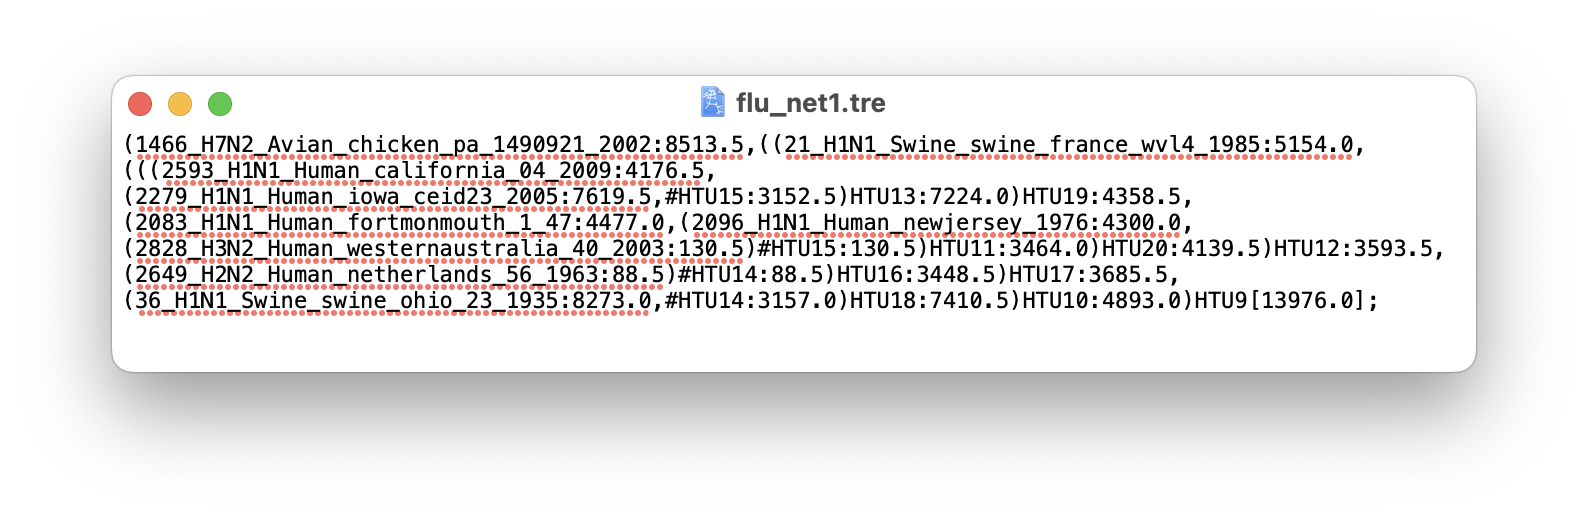
\includegraphics[width=\textwidth]{tre1.png}
\caption{Output file \textbf{``flu\_net1.tre''} in ENewick graph format.}
\label{tre1}
\end{figure}

\item  The command \texttt{report("filename.tre", dotpdf, graphs, overwrite)} will 
produce a file that can be read in \textit{Adobe Illustrator}, \textit{Apple Preview} 
or any vectorial image editor program. Notice that two files were outputted from 
using this command. \phyg has output an eps (on OSX) or pdf (on linux) file that 
can be viewed in a vector graphics program and a dot file, which can be viewed 
(and modified) in \textit{Graphviz}. Note: in order to output pdf files the application 
\textit{dot} must be installed from the \href{https://graphviz.org/download/}{Graphviz} 
website. \textit{dot} is a graph description language and Graphviz an open-source 
graph visualization software. This program is well suited to representing graphs 
and networks. Open the reported file \textbf{``flu\_net1\_gv.tre.eps''} in your preferred
visualization program (Figure \ref{eps1}). The values associated with the taxon 
names and HTUs are the branch lengths. Examining this file, we can see two
networks (one leading into HTU14 and HTU15).

\begin{figure}[H]
\centering
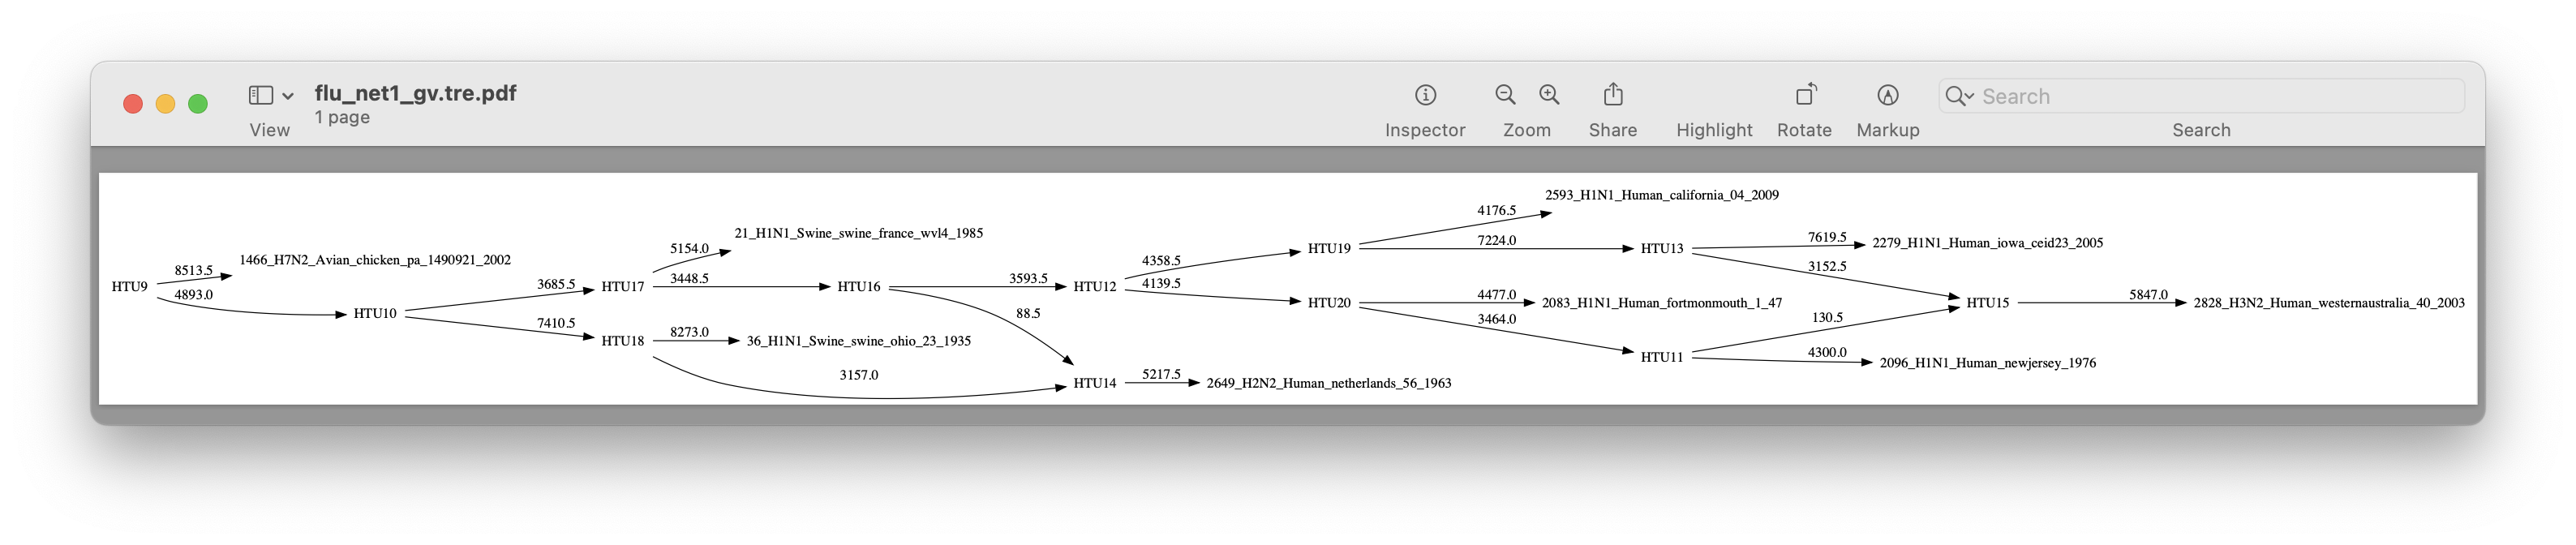
\includegraphics[width=\textwidth]{eps1.png}
\caption{Output file \textbf{``flu\_net1\_gv.tre.eps''} in eps format.}
\label{eps1}
\end{figure}

\end{enumerate}
%-------------------------------------------------------------------------------------------------------
\subsection{Refining a softwired network: adding network edges}
\label{subsec:netadd}

Now that we have a network to work with, we can do some refinement operations 
on the network edges. In the next five tutorials we will learn how to perform 
manipulation of network edges to existing network graphs. This tutorial will 
focus on adding network edges.

\begin {enumerate}

\item Rather than modify the previous script (possible to do with comments and 
additional text), we will generate a new script to perform the refinements of our
first network.

\item Open your text editor of choice and type the following:

	\begin{quote}	
	-\/-Refinements of softwired networks using flu data sets using netadd\\
	set(seed:1634561640)\\
	set(outgroup:"1466\_H7N2\_Avian\_chicken\_pa\_1490921\_2002")\\
	set(graphtype:softwired)\\
	set(graphfactor:w15)\\ 
	read(nucleotide:"flu*.fas*", tcm:(2,1))\\
	read(newick:"flu\_net1.tre")\\
	refine(netadd, maxnetedges:5, atrandom, steepest)\\
	report("flu\_net2.tre", graphs, newick, overwrite)\\
	report("flu\_net2\_gv.tre", dotpdf, graphs, overwrite)
	\end{quote}

\item The script begins with a comment that describes the purpose of this 
analysis.

\item The next three lines are identical to that of \textbf{``flu\_net1.pg''}, so we 
will not comment about them any further. 

\item Unlike the previous script, here, we \texttt{set} the \texttt{graphfactor} to 
\texttt{w15}. This penalty involves the calculation of the most parsimonious 
display tree. `Softwired' networks monotonically reduce the network cost 
with each additional network edge. A display tree is a tree created from a 
`softwired' graph by deleting one of two of the network edges incident on 
network vertex. Because this penalty has a higher time complexity to calculate 
the total network costs (than \texttt{w23} and \texttt{nopenalty}), this may take 
significantly more time for larger datasets. 

\item In addition to importing the nucleotide sequence data files, we also
read in the \texttt{newick} graph file \textbf{``flu\_net1.tre''} generated from the 
previous tutorial (Section \ref{subsec:makinganetwork}). Reading in tree or graph 
files, rather than building them from scratch, can be a useful starting point and 
can speed up analyses.

\item Having \texttt{read} in our data and graph files, we can now perform refinements 
of the network. The command \texttt{refine} performs edit operations on network 
edges. The network specific refinement operations include \texttt{netadd}, 
\texttt{netdel}, \texttt{netadddel} and \texttt{netmove}. These refinements are 
only applicable to network edges, hence they can only be applied to `softwired' 
and `hardwired' graphs (as opposed to trees). \\

The argument \texttt{netadd} adds network edges to input graphs at all possible
positions until no better cost graph is found. Though no need to specify here as
they are the default arguments of \texttt{refine}, we specify \texttt{atrandom} and 
\texttt{steepest}. \texttt{atrandom} randomizes the evaluation of the networks and 
the order by which they are generated. \texttt{steepest} specifies that if a better 
network is found during the network refinement operations then the refinements 
will switch greedily to this graph and abandon the previous network. The argument  
\texttt{maxnetedges:n} specifies that network edges can only be added to networks 
with the number of edges less that the specified integer \texttt{n}. This can only be 
used in conjunction with \texttt{netadd} and \texttt{netadddel}.

\item Save this file with the name \textbf{``flu\_net2.pg''} in the same directory as the 
data files and previously reported graph files.

\item Run the script.

\begin{figure}
\centering
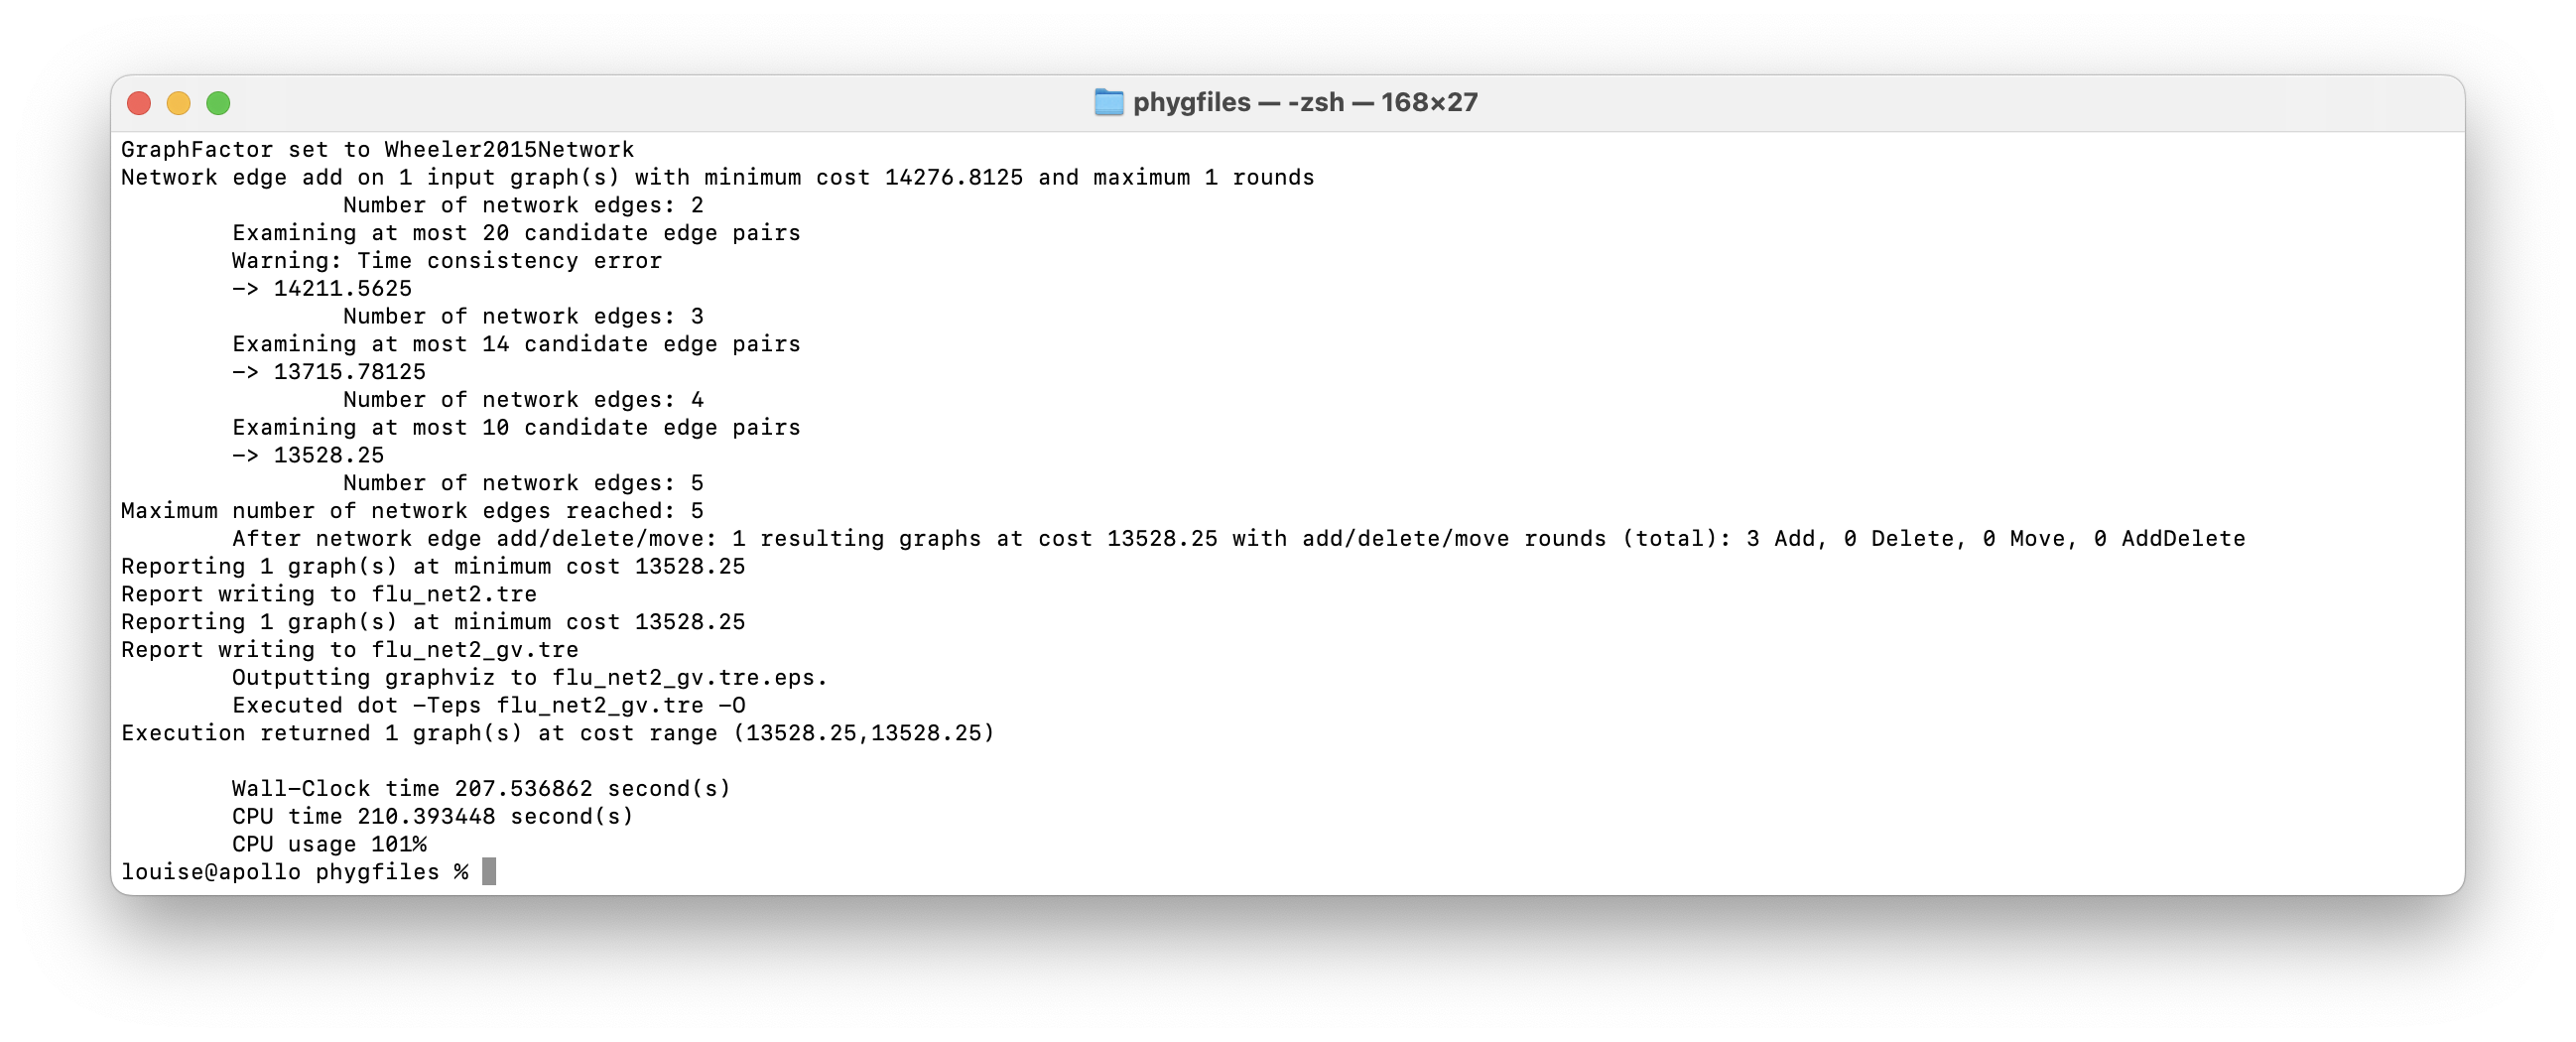
\includegraphics[width=\textwidth]{output1.png}
\caption{Output of the \textit{Terminal} window from running the script 
\textbf{``flu\_net2.pg''}.}
\label{output1}
\end{figure}

\item Scroll through the output in the \textit{Terminal} window (Figure \ref{output1}). 
Having \texttt{read} in the data files, they were then processed or transformed using 
the \texttt{tcm} information. The blocks of characters (in this case the data files) were 
recoded in that \phyg is processing the data. Then the settings of \phyg were \texttt{set}. 
Note: the cost of the input graph \textbf{``flu\_net1.tre''} has increased from 13976 to 
14276.8125. Recall that this graph was generated under \texttt{nopenalty} costs and 
here the penalty is \texttt{set} to \texttt{w15}. Therefore, when this graph is read in, it 
is rediagnosed with the new penalty cost. \phyg then performed 3 rounds of adding 
network edges, examining a decreasing number of candidate edge pairs after each 
round. As you add network edges the number of possible new edges will go down 
(in most cases) because of the constrains of phylogenetic networks. In each round 
\phyg added a network edge. \phyg stopped after three rounds as we specified 
\texttt{maxnetedges:5}. Notice the reduction in network cost after each round. Note:
the message ``Warning: Time consistency error'' is an internal processing error and 
can be ignored.\\

Let's examine the reported graph files. 

\item Opening the file \textbf{``flu\_net2.tre''} in your preferred text editor (Figure 
\ref{tre2}). This ENewick file has ten \textbf{\#}'s, representing the reticulation events. 
Comparing this graph to \textbf{``flu\_net1.tre''} (our input graph), we can see that 
the addition of three additional network edges, reduced the cost of the network from 
14276.8125 to 13528.25. 

\begin{figure}[H]
\centering
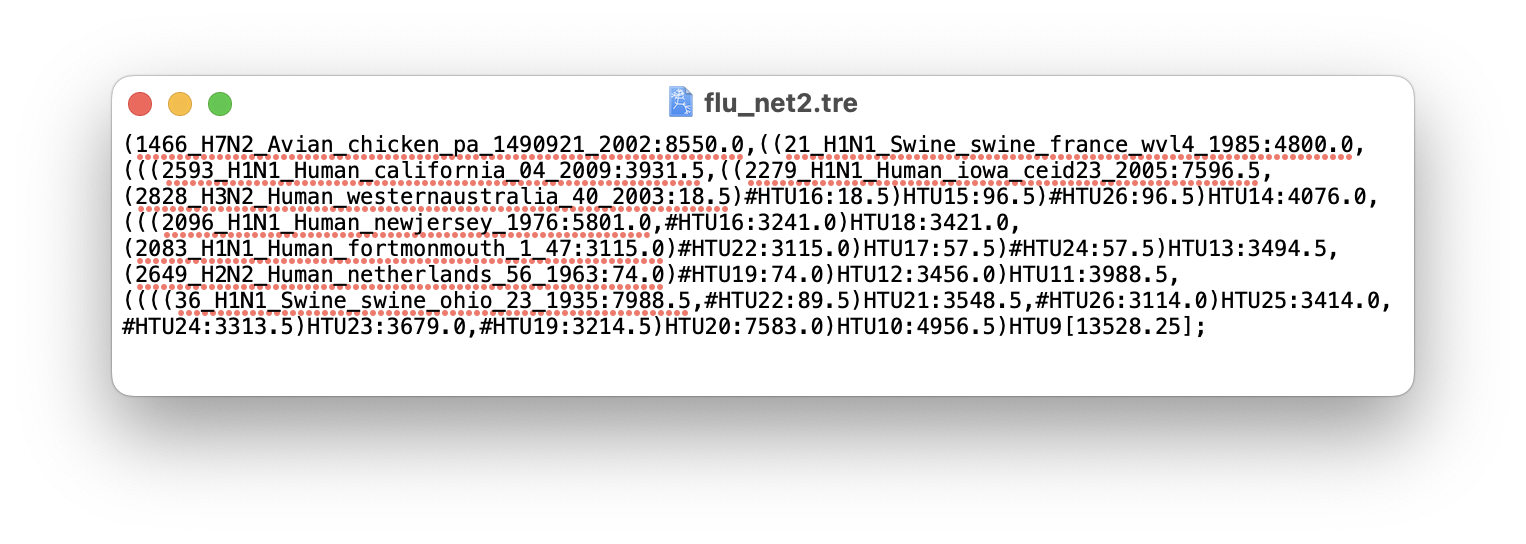
\includegraphics[width=\textwidth]{tre2.png}
\caption{Output file \textbf{``flu\_net2.tre''} in ENewick graph format.}
\label{tre2}
\end{figure}

\item  Open the reported file \textbf{``flu\_net2\_gv.tre.eps''}  in your preferred
visualization program (Figure \ref{eps2}). The values associated with the taxon 
names and HTUs are the branch lengths. Examining this file, we can see five 
networks (one leading into HTU19, HTU24, HTU26, HTU22 and HTU16). A single
graph was reported.

\begin{figure}[H]
\centering
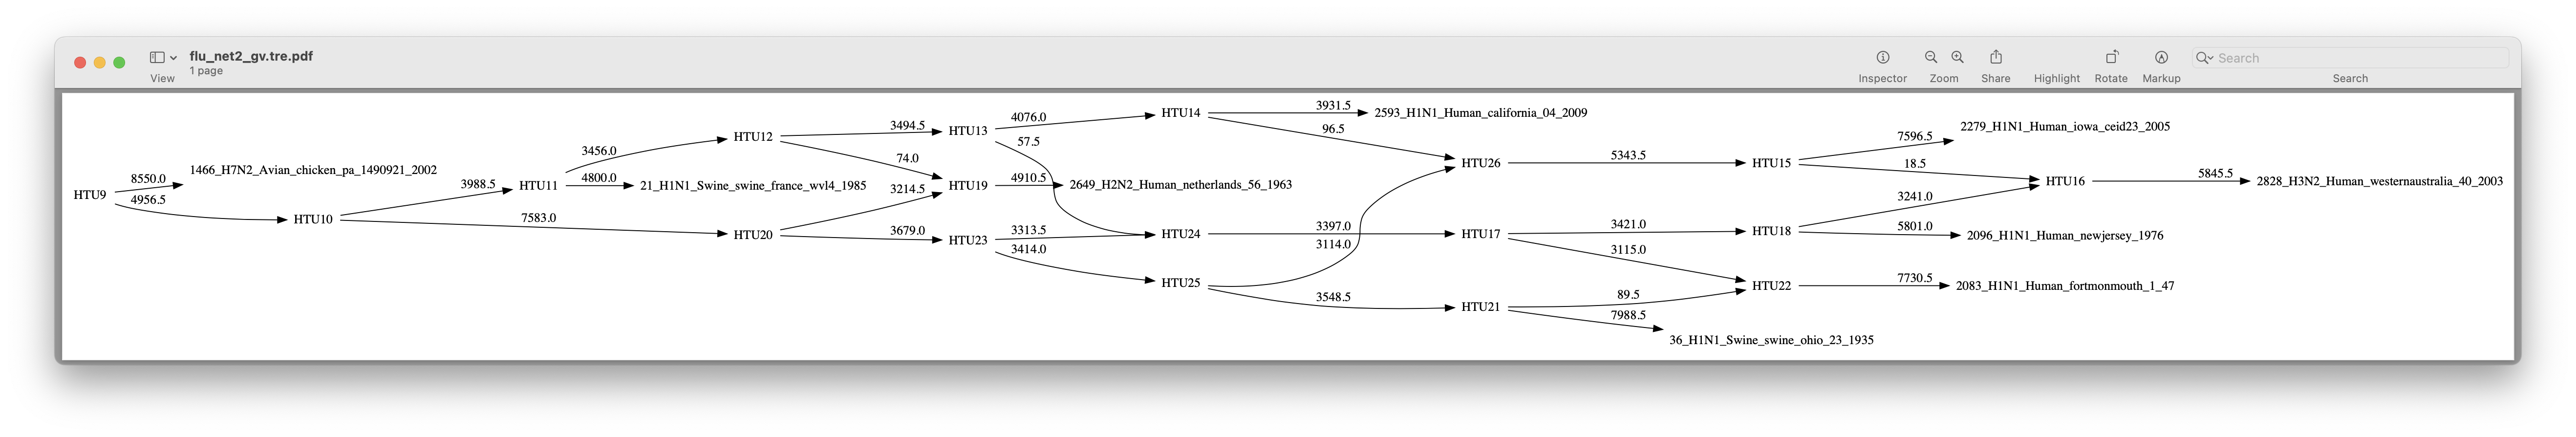
\includegraphics[width=\textwidth]{eps2.png}
\caption{Output file \textbf{``flu\_net2\_gv.tre.eps''} in eps format.}
\label{eps2}
\end{figure}

\item We can apply some of the commands that we learned in Tutorial 0.1 to
these tutorials. As we learned previously, another useful way to visualize the data 
is to \texttt{report} the implied alignment of the molecular data currently loaded. 
The implied alignment is a visual representation (alignment) of the indel and 
substitution events that take place on a \textit{given} graph. \\

Modify the script to include the following: 

\begin{quote}
report("flu\_net2\_ia.ss", ia, overwrite)
\end{quote}

This command will output an implied alignment for each reported graph, as well as 
for each block of imported data. 

%Should you wish to output an implied alignment
%that is readable by the program \textit{TNT}, you should modify the command  
%replacing \texttt{ia} with the argument \texttt{tnt}.
%
%\begin{quote}
%report("flu\_net2\_ia.ss", tnt, overwrite)
%\end{quote}

\end{enumerate}

%-------------------------------------------------------------------------------------------------------
\subsection{Refining a softwired network: deleting network edges}
\label{subsec:netdel}

This tutorial will focus on deleting network edges.

\begin {enumerate}

\item Open your text editor of choice and type the following:

	\begin{quote}	
	-\/-Refinements of softwired networks using flu data sets using netdel\\
	set(seed:1634561640)\\
	set(outgroup:"1466\_H7N2\_Avian\_chicken\_pa\_1490921\_2002")\\
	set(graphtype:softwired)\\
	set(graphfactor:w15)\\ 
	read(nucleotide:"flu*.fas*", tcm:(2,1))\\
	read(newick:"flu\_net1.tre")\\
	refine(netdel, atrandom, steepest)\\
	report("flu\_net3.tre", graphs, newick, overwrite)\\
	report("flu\_net3\_gv.tre", dotpdf, graphs, overwrite)
	\end{quote}

\item The script begins with a comment that describes the purpose of this 
analysis.

\item The next six lines are identical to that of \textbf{``flu\_net1.pg''}, so we 
will not comment about them any further. 

\item Having \texttt{read} in our data and graph files, we can now perform 
refinements of the network. The argument \texttt{netdel} deletes network edges 
from input graphs one at a time until no better cost graph is found. We also 
specify that this edit operation be performed using \texttt{atrandom} and 
\texttt{steepest}.

\item Save this file with the name \textbf{``flu\_net3.pg''} in the same directory 
as the data files and previously reported graph files.

\item Run the script.

\begin{figure}[H]
\centering
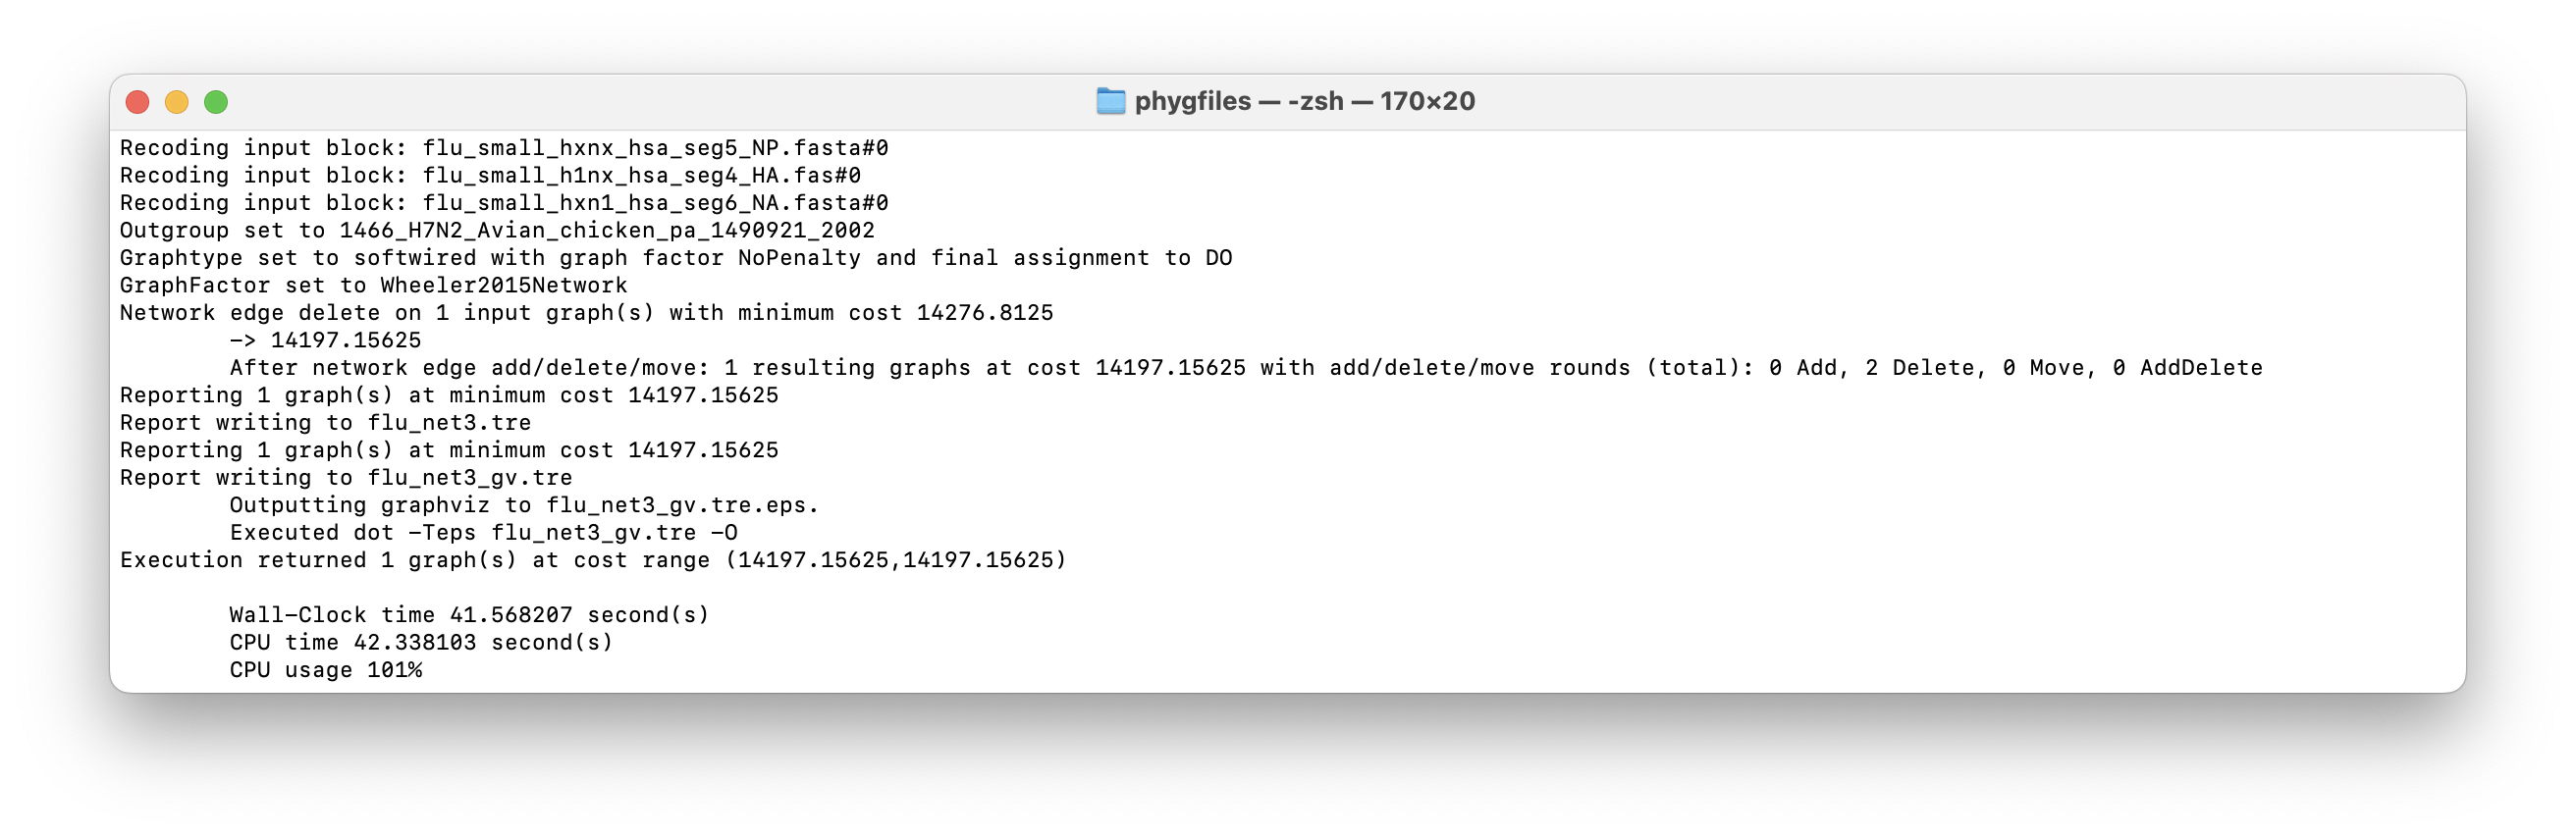
\includegraphics[width=\textwidth]{output2.png}
\caption{Output of the \textit{Terminal} window from running the script 
\textbf{``flu\_net3.pg''}.}
\label{output2}
\end{figure}

\item Scroll through the output in the \textit{Terminal} window (Figure \ref{output2}). 
Having \texttt{read} in the data files, they were then processed and the settings of 
\phyg were \texttt{set}. The output for \texttt{netdel} looks different to that of 
\texttt{netadd}---the recursive output is not show---as \texttt{netdel} is not dependent 
on the maximum number of edges, as is the case with \texttt{netadd}. \phyg performed 
2 rounds of deleting network edges, but it could only delete one network edge.\\

Let's examine the reported graph files. 

\item Opening the file \textbf{``flu\_net3.tre''} in your preferred text editor. This 
ENewick file has two \textbf{\#}'s, representing the reticulation events (Figure 
\ref{tre3}). Comparing this graph to \textbf{``flu\_net1.tre''} (our input graph), we can 
see that the deletion of one network edge, reduced the cost of the network from 
14276.8125 to 14197.15625. A single graph was reported.

\begin{figure}[H]
\centering
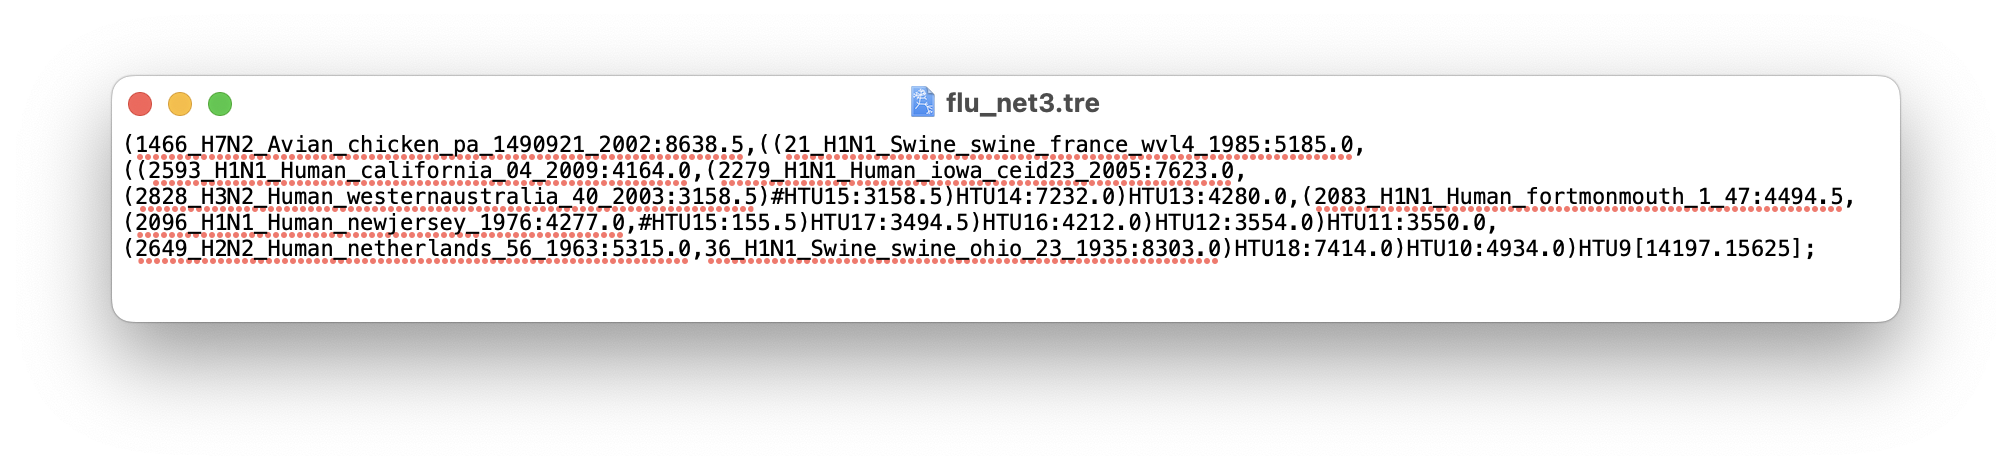
\includegraphics[width=\textwidth]{tre3.png}
\caption{Output file \textbf{``flu\_net3.tre''} in ENewick graph format.}
\label{tre3}
\end{figure}

\item  Open the reported file \textbf{``flu\_net3\_gv.tre.eps''} in your preferred
visualization program (Figure \ref{eps3}). The values associated with the taxon 
names and HTUs are the branch lengths. Examining this file, we can see a single
network leading to HTU15.

\begin{figure}[H]
\centering
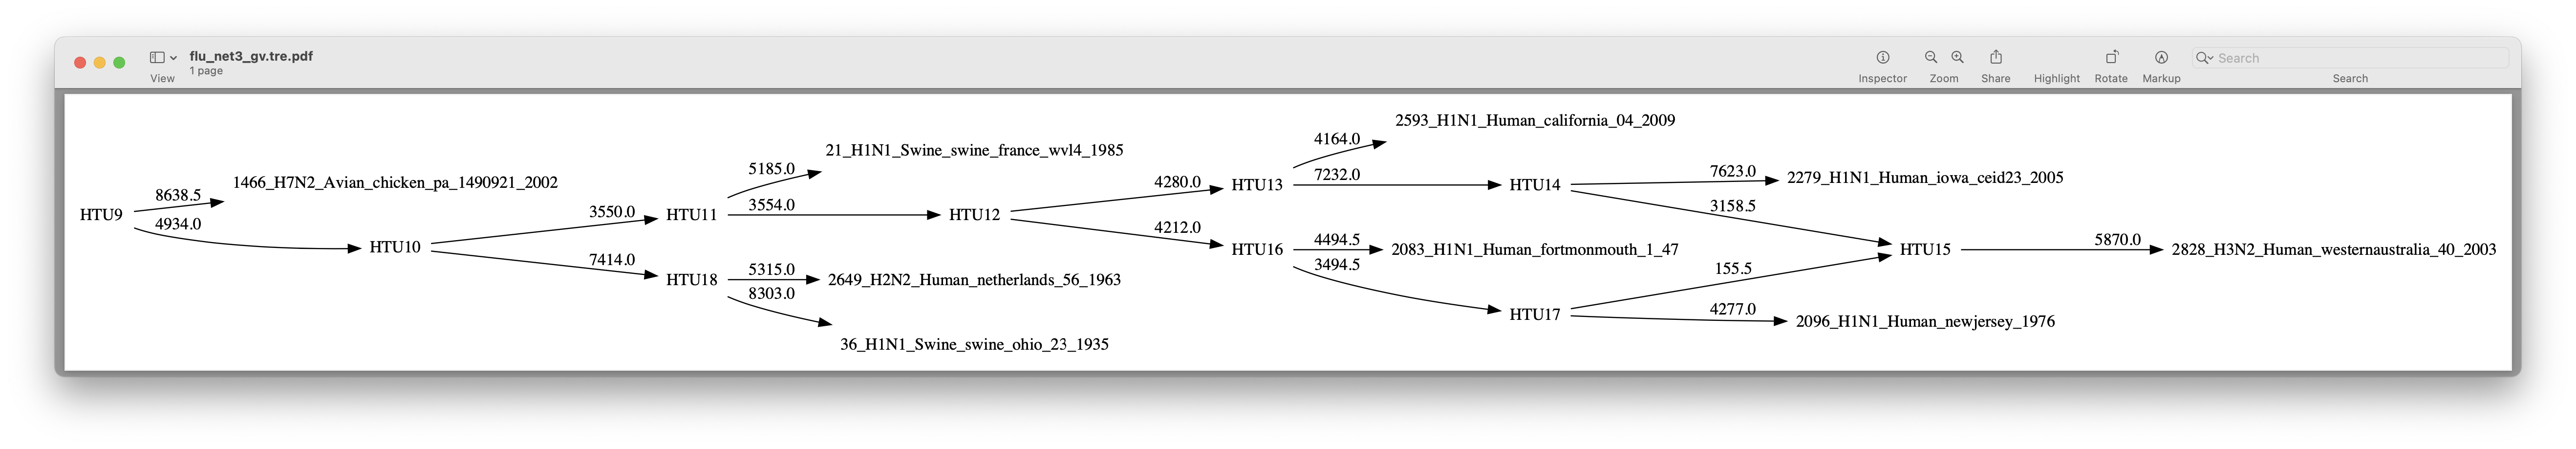
\includegraphics[width=\textwidth]{eps3.png}
\caption{Output file \textbf{"flu\_net3\_gv.tre.eps"} in eps format.}
\label{eps3}
\end{figure}

\item In this tutorial we read in the input graph \textbf{``flu\_net1.tre''}. What 
happens if instead we read in \textbf{``flu\_net2.tre''}, our graph from our 
\texttt{netadd} operation? \\

Modify the script using comments and new output file names.
	
\item Rerun the script.

\item Answer the following questions: 
\subitem Does this change the number of resulting networks?
\subitem How does changing the input graph affected the cost of the graph?

\end{enumerate}
%-------------------------------------------------------------------------------------------------------
\subsection{Refining a softwired network: adding and deleting network edges}
\label{subsec:netadddel}

This tutorial will focus on consecutively adding and deleting network edges.

\begin {enumerate}

\item Open your text editor of choice and type the following:
	
	\begin{quote}	
	-\/-Refinements of softwired networks using flu data sets using netadddel\\
	set(seed:1634561640)\\
	set(outgroup:"1466\_H7N2\_Avian\_chicken\_pa\_1490921\_2002")\\
	set(graphtype:softwired)\\
	set(graphfactor:w15)\\ 
	read(nucleotide:"flu*.fas*", tcm:(2,1))\\
	read(newick:"flu\_net1.tre")\\
	refine(netadddel, maxnetedges:5, atrandom, steepest)\\
	report("flu\_net4.tre", graphs, newick, overwrite)\\
	report("flu\_net4\_gv.tre", dotpdf, graphs, overwrite)
	\end{quote}

\item The script begins with a comment that describes the purpose of this 
analysis.

\item The next six lines are identical to that of \textbf{``flu\_net1.pg''}, so we 
will not comment about them any further. 

\item Having \texttt{read} in our data and graph files, we can now perform 
refinements of the network. The argument \texttt{netadddel} consecutively 
adds and then deletes network edges from input graphs until certain conditions
are met. In this case, until either no improvement (graph cost) is found
in each round or until the number of edges (in \texttt{maxnetedges:n}) is reached. 
It does so until whichever condition comes first. The deletion of network edges 
does not occur until the addition of network edges has satisfied these condition.
We also specify that this edit operation be performed using \texttt{atrandom} 
and \texttt{steepest}.

\item Save this file with the name \textbf{``flu\_net4.pg''} in the same directory 
as the data files and previously reported graph files.

\item Run the script.

\begin{figure}[H]
\centering
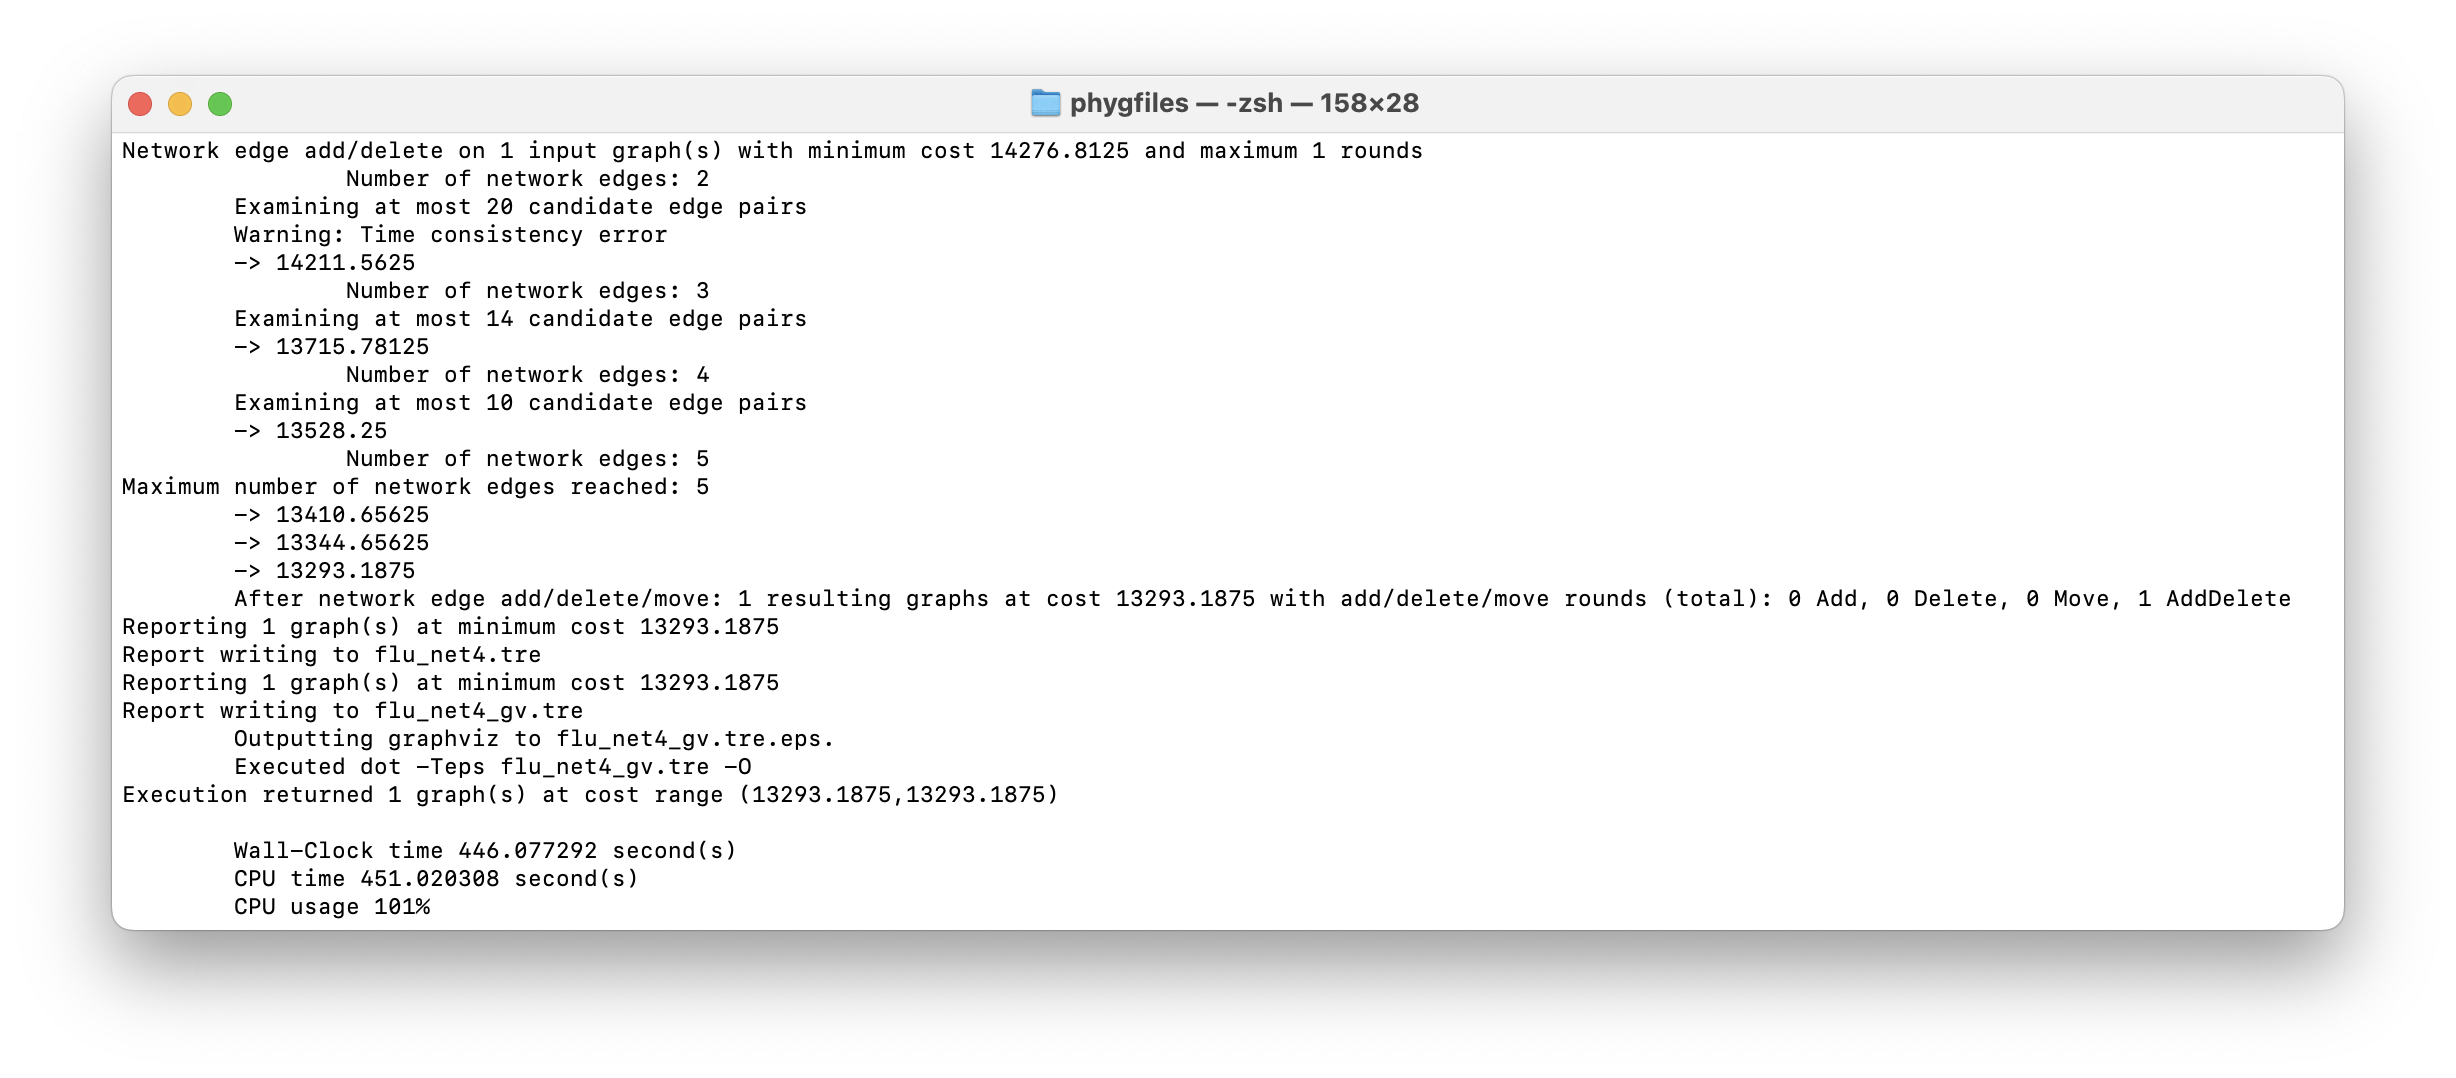
\includegraphics[width=\textwidth]{output3.png}
\caption{Output of the \textit{Terminal} window from running the script 
\textbf{``flu\_net4.pg''}.}
\label{output3}
\end{figure}

\item Scroll through the output in the \textit{Terminal} window (Figure \ref{output3}). 
Having \texttt{read} in the data files, they were then processed and the settings of 
\phyg were \texttt{set}. The recursive output is shown. \phyg performed a single 
round of addition, followed by deletion operations of network edges. The cost of 
the graph continues to decrease with each edit operation a network edge. A single 
round is the default for \texttt{netadddel}.\\

Let's examine the reported graph files. 

\item Opening the file \textbf{``flu\_net4.tre''} in your preferred text editor. This 
ENewick file has eight \textbf{\#}'s, representing the reticulation events (Figure 
\ref{tre4}). Comparing this graph to \textbf{``flu\_net1.tre''} (our input graph from 
Section \ref{subsec:makinganetwork}), we can see that the deletion of one network 
edge, reduced the cost of the network from 14276.8125 to 13293.187. A single graph 
was reported.

\begin{figure}[H]
\centering
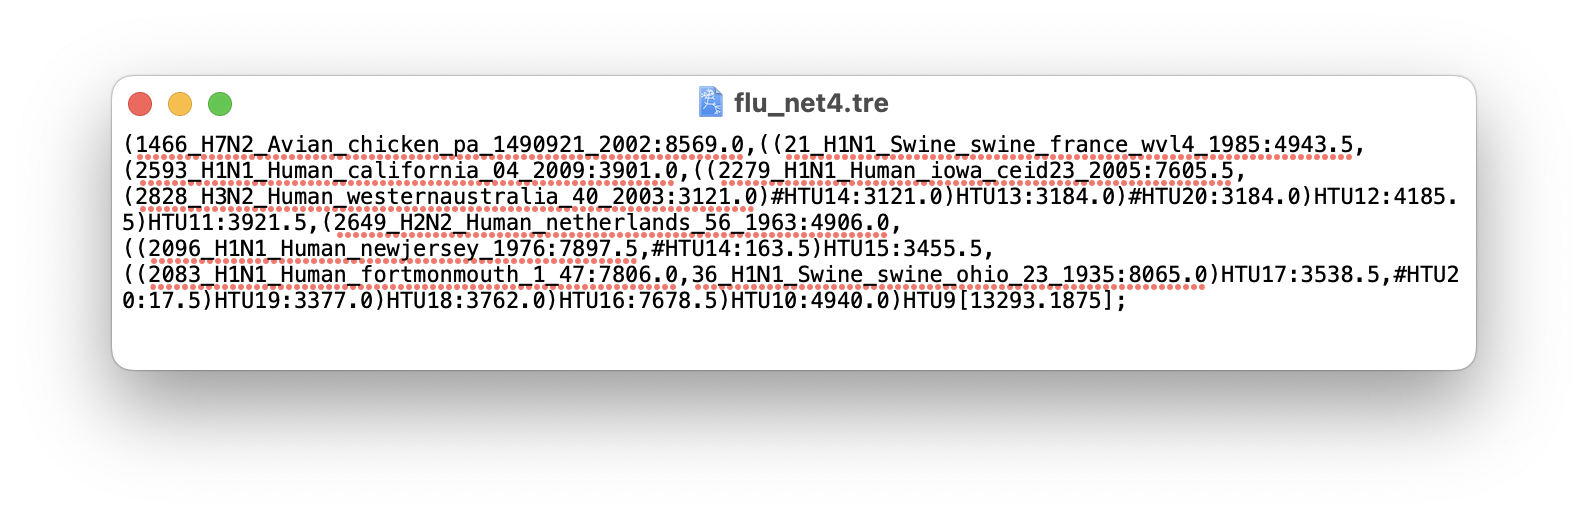
\includegraphics[width=0.8\textwidth]{tre4.png}
\caption{Output file \textbf{``flu\_net4.tre''} in ENewick graph format.}
\label{tre4}
\end{figure}

\item  Open the reported file \textbf{``flu\_net4\_gv.tre.eps''} in your preferred
visualization program (Figure \ref{eps4}). The values associated with the taxon 
names and HTUs are the branch lengths. Examining this file, we can see a four
networks leading to HTU22, HTU20, HTU14 and HTU24.

\begin{figure}[H]
\centering
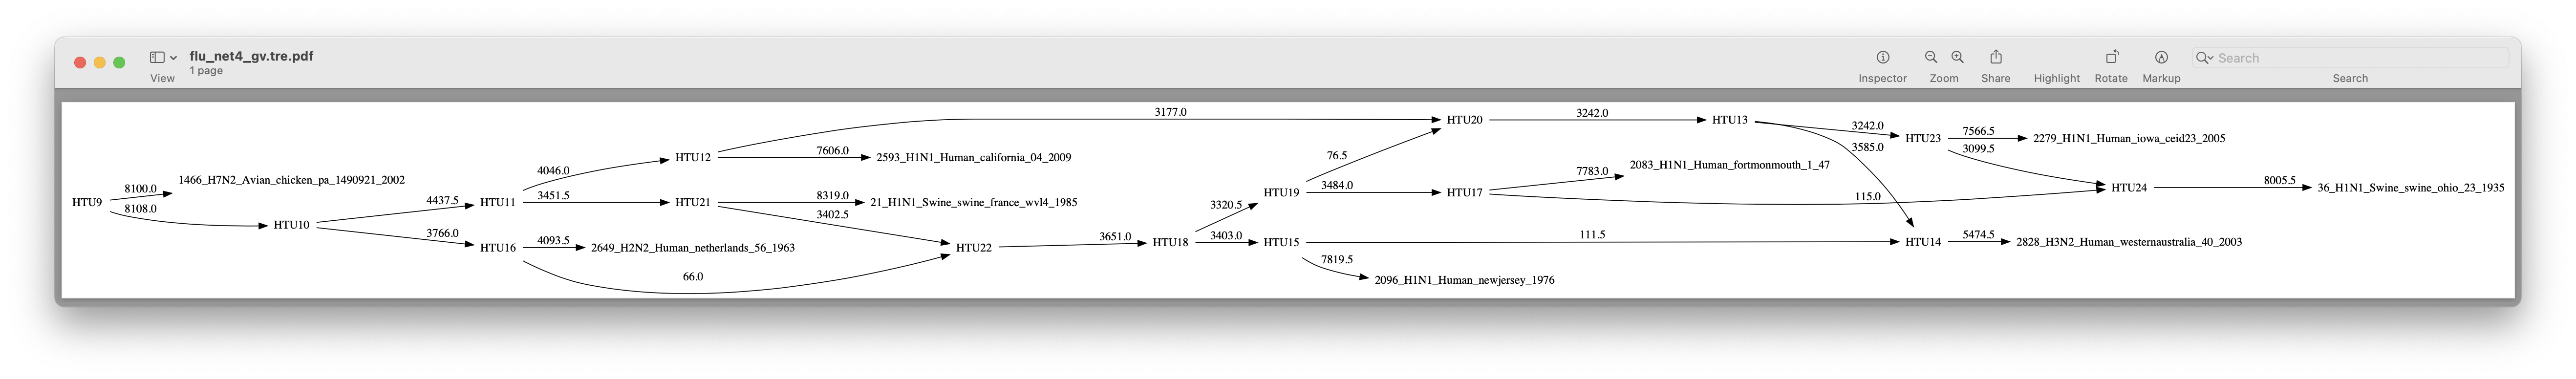
\includegraphics[width=\textwidth]{eps4.png}
\caption{Output file \textbf{"flu\_net4\_gv.tre.eps"} in eps format.}
\label{eps4}
\end{figure}

\item In this tutorial we used the default setting for \texttt{netadddel}, which 
included performing a single round of edit operations. What would happen 
if we increase the number of rounds of netadddel operations that \phyg 
performs? \\

Modify the script as follows:

	\begin{quote}
	refine(netadddel, maxnetedges:5, atrandom, steepest, rounds:2)
	\end{quote}
	
\item Rerun the script.

\item Answer the following questions: 
\subitem Does this change the number of resulting networks?
\subitem How does increasing the number of operation rounds affected the 
cost of the tree?
\subitem How does this cost compare to that of the graphs from the previous 
tutorial (Section \ref{subsec:netdel})?

\end{enumerate}
%-------------------------------------------------------------------------------------------------------
\subsection{Refining a softwired network: moving network edges}
\label{subsec:softnetmove}

This tutorial focuses on moving network edges.

\begin {enumerate}

\item Open your text editor of choice and type the following:

	\begin{quote}	
	-\/-Refinements of softwired networks using flu data sets using netmove\\
	set(seed:1634561640)\\
	set(outgroup:"1466\_H7N2\_Avian\_chicken\_pa\_1490921\_2002")\\
	set(graphtype:softwired)\\
	set(graphfactor:w15)\\ 
	read(nucleotide:"flu*.fas*", tcm:(2,1))\\
	read(newick:"flu\_net1.tre")\\
	refine(netmove, atrandom, steepest)\\
	report("flu\_net5.tre", graphs, newick, overwrite)\\
	report("flu\_net5\_gv.tre", dotpdf, graphs, overwrite)
	\end{quote}

\item The script begins with a comment that describes the purpose of this 
analysis.

\item The next six lines are identical to that of \textbf{``flu\_net1.pg''}, so we 
will not comment about them any further. 

\item Having \texttt{read} in our data and graph files, we can now perform 
refinements of the network. The argument \texttt{netmove} moves existing 
network edges in input graphs one at a time to new positions until there
are no more improvements in the cost of the graph. We also specify that 
this edit operation be performed using \texttt{atrandom} and \texttt{steepest}.

\item Save this file with the name \textbf{``flu\_net5.pg''} in the same directory 
as the data files and previously reported graph files.

\item Run the script.

\begin{figure}[H]
\centering
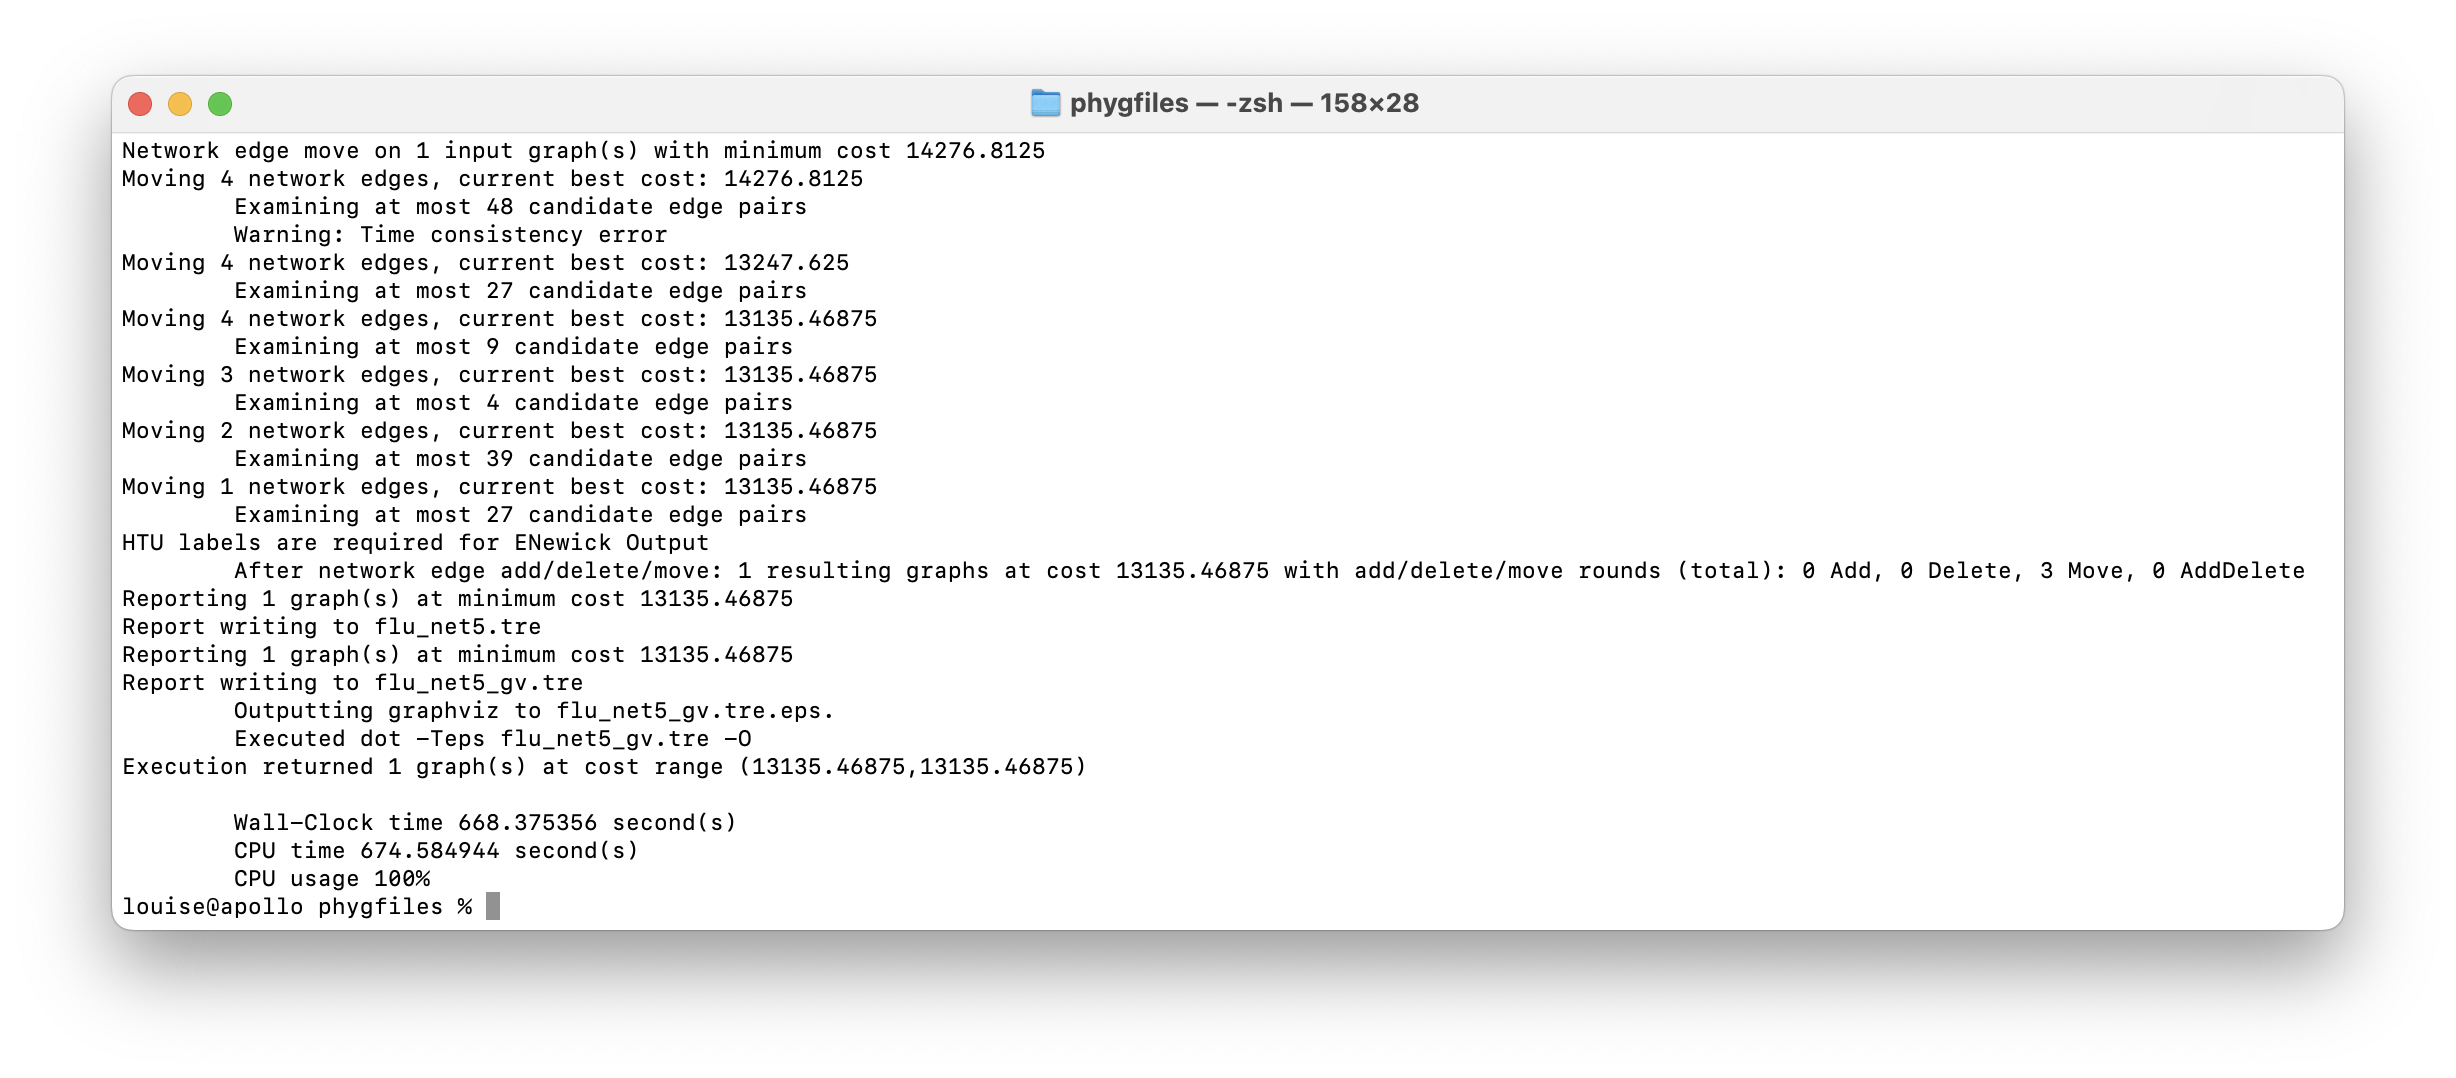
\includegraphics[width=\textwidth]{output4.png}
\caption{Output of the \textit{Terminal} window from running the script 
\textbf{``flu\_net5.pg''}.}
\label{output4}
\end{figure}

\item Scroll through the output in the \textit{Terminal} window (Figure \ref{output4}). 
Having \texttt{read} in the data files, they were then processed and the settings of 
\phyg were \texttt{set}. \phyg performed three round of moves of network edges.
We can see that \phyg did three full rounds of moves, with the cost decreasing 
with each move.\\

Let's examine the reported graph files. 

\item Opening the file \textbf{``flu\_net5.tre''} in your preferred text editor. This 
ENewick file has four \textbf{\#}'s, representing the vertices (Figure \ref{tre5}). 
Comparing this graph to \textbf{``flu\_net1.tre''} (our input graph), we can see 
that \phyg the moves reduced the cost of the network from 14276.8125 to 
13135.46875. A single graph was reported. With \texttt{netmove} the number 
of network edges/vertices is maintained between the input and output graphs.

\begin{figure}[H]
\centering
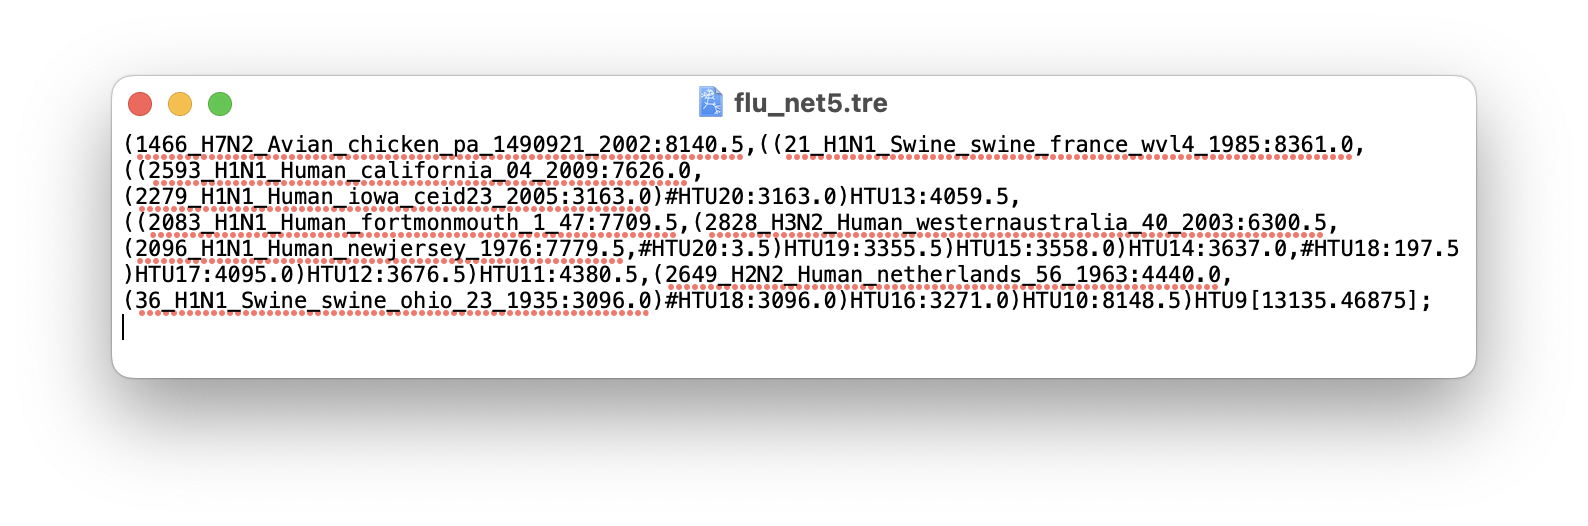
\includegraphics[width=0.8\textwidth]{tre5.png}
\caption{Output file \textbf{``flu\_net5.tre''} in ENewick graph format.}
\label{tre5}
\end{figure}

\item  Open the reported file \textbf{``flu\_net5\_gv.tre.eps''} in your preferred
visualization program (Figure \ref{eps5}). The values associated with the taxon 
names and HTUs are the branch lengths. Examining this file, we can see a four
networks leading to HTU18 and HTU20.

\begin{figure}[H]
\centering
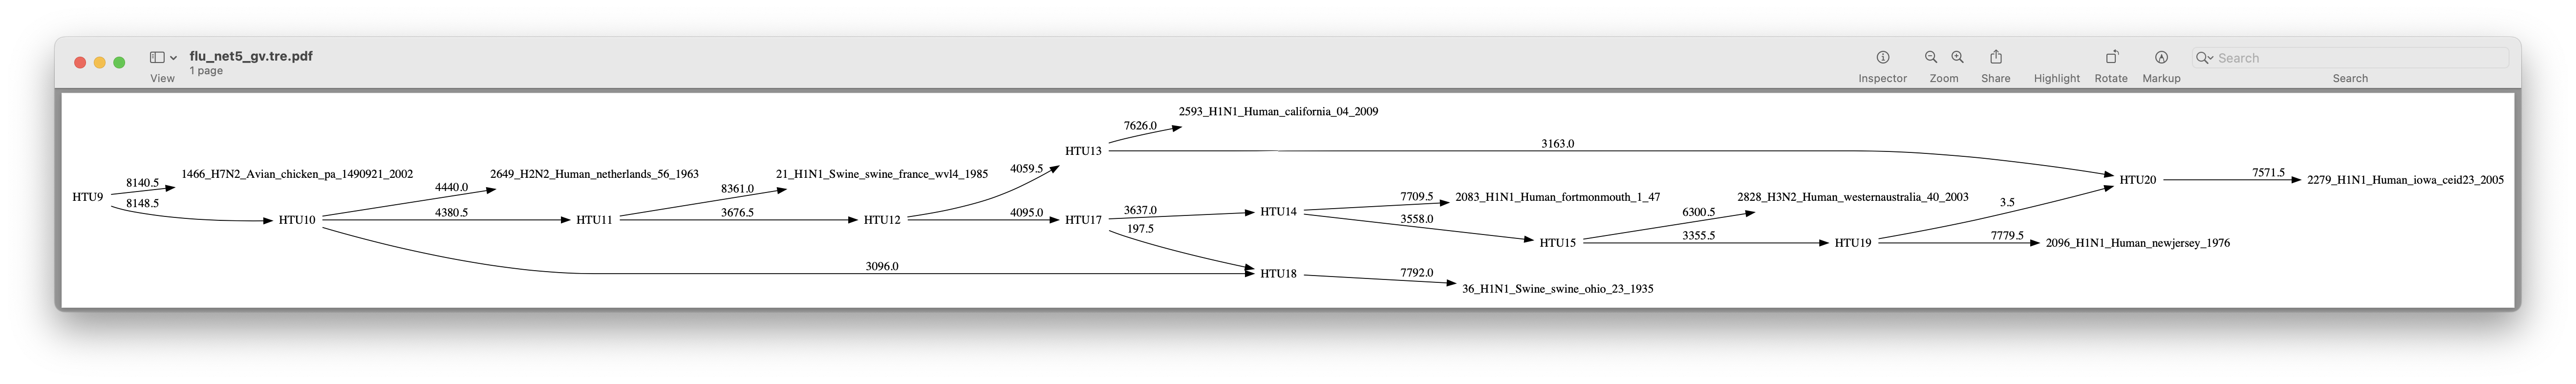
\includegraphics[width=\textwidth]{eps5.png}
\caption{Output file \textbf{"flu\_net5\_gv.tre.eps"} in eps format.}
\label{eps5}
\end{figure}

\item One of the output option for `softwired' networks is to report the `display' 
trees. Recall that a `display' tree or `tree-based network' is a tree created from 
a `softwired' graph by deleting one of two of the network edges/vertices. Modify 
the script to include \texttt{report("flu\_net5\_dt.tre", displaytrees, newick, 
overwrite)}.

\item Run the updated script.

\item Examine the reported file.  For now `display' trees can only be reported
in newick format (as opposed to dotpdf and eps format---the error lies with \textit{dot}
on OSX machines). This newick tree file, in parenthetical notation, can be viewed in 
other programs like \textit{FigTree} or \textit{TreeView}.

%\item In Tutorial 0.1 we learned how to perform a local search on the graphs stored 
%in memory. Let's do that here. Modify the script to include \texttt{swap(spr:3)}.
%This command specifies that SPR refinement \citep{Dayhoff1969} is performed. 
%Because we specify the optional argument \texttt{n}, the readdition of pruned graphs 
%will be within $2 * N$ edges of its original placement.
%
%\item Run the modified script.
%
%\item Now reexamine the reported file \textbf{``flu\_net5.tre''}. Notice that this 
%simple local search has reduced the cost of the initial best tree from 13135.46875
%to \hl{xxx}.

\end{enumerate}
%-------------------------------------------------------------------------------------------------------
\subsection{Hardwired network: moving network edges}
\label{subsec:hardnetmove}

So far, the tutorials have centered on `softwired' graphs. In this tutorial, we will 
focus of `hardwired' graphs.

\begin {enumerate}

\item Open your text editor of choice and type the following:

	\begin{quote}	
	-\/-Refinements of hardwired networks using flu data sets using netmove\\
	set(seed:1634561640)\\
	set(outgroup:"1466\_H7N2\_Avian\_chicken\_pa\_1490921\_2002")\\
	set(graphtype:hardwired)\\
	read(nucleotide:"flu*.fas*", tcm:(2,1))\\
	read(newick:"flu\_net1.tre")\\
	refine(netmove, atrandom, steepest)\\
	report("flu\_net6.tre", graphs, newick, overwrite)\\
	report("flu\_net6\_gv.tre", dotpdf, graphs, overwrite)
	\end{quote}
	
\item The script begins with a comment that describes the purpose of this 
analysis.

\item The next two lines are identical to that of \textbf{``flu\_net1.pg''}, so we 
will not comment about them any further. 	

\item We next \texttt{set} the \texttt{graphtype} of this analysis to \texttt{hardwired}. 

\item When conducting a `hardwired' network analysis, there is no need to \texttt{set}
a \texttt{graphfactor} or penalty cost. Unlike `softwired networks', which discussed, 
monotonically reduces the network cost with each additional network edge, 
the cost of `hardwired' networks monotonically increases with the addition of each 
additional network edge. By extension, the number of network edges is kept constant
with \texttt{netmove}, so there is no need to ascribe a penalty cost.

\item In addition to importing the nucleotide sequence data files, we also read in 
the \texttt{newick} graph file \textbf{``flu\_net1.tre''}.

\item The argument \texttt{netmove} moves network edges on the input graphs 
to all possible positions until no better cost graph is found. We also specify 
\texttt{atrandom} and \texttt{steepest}.

\item Rerun the script.

\begin{figure}
\centering
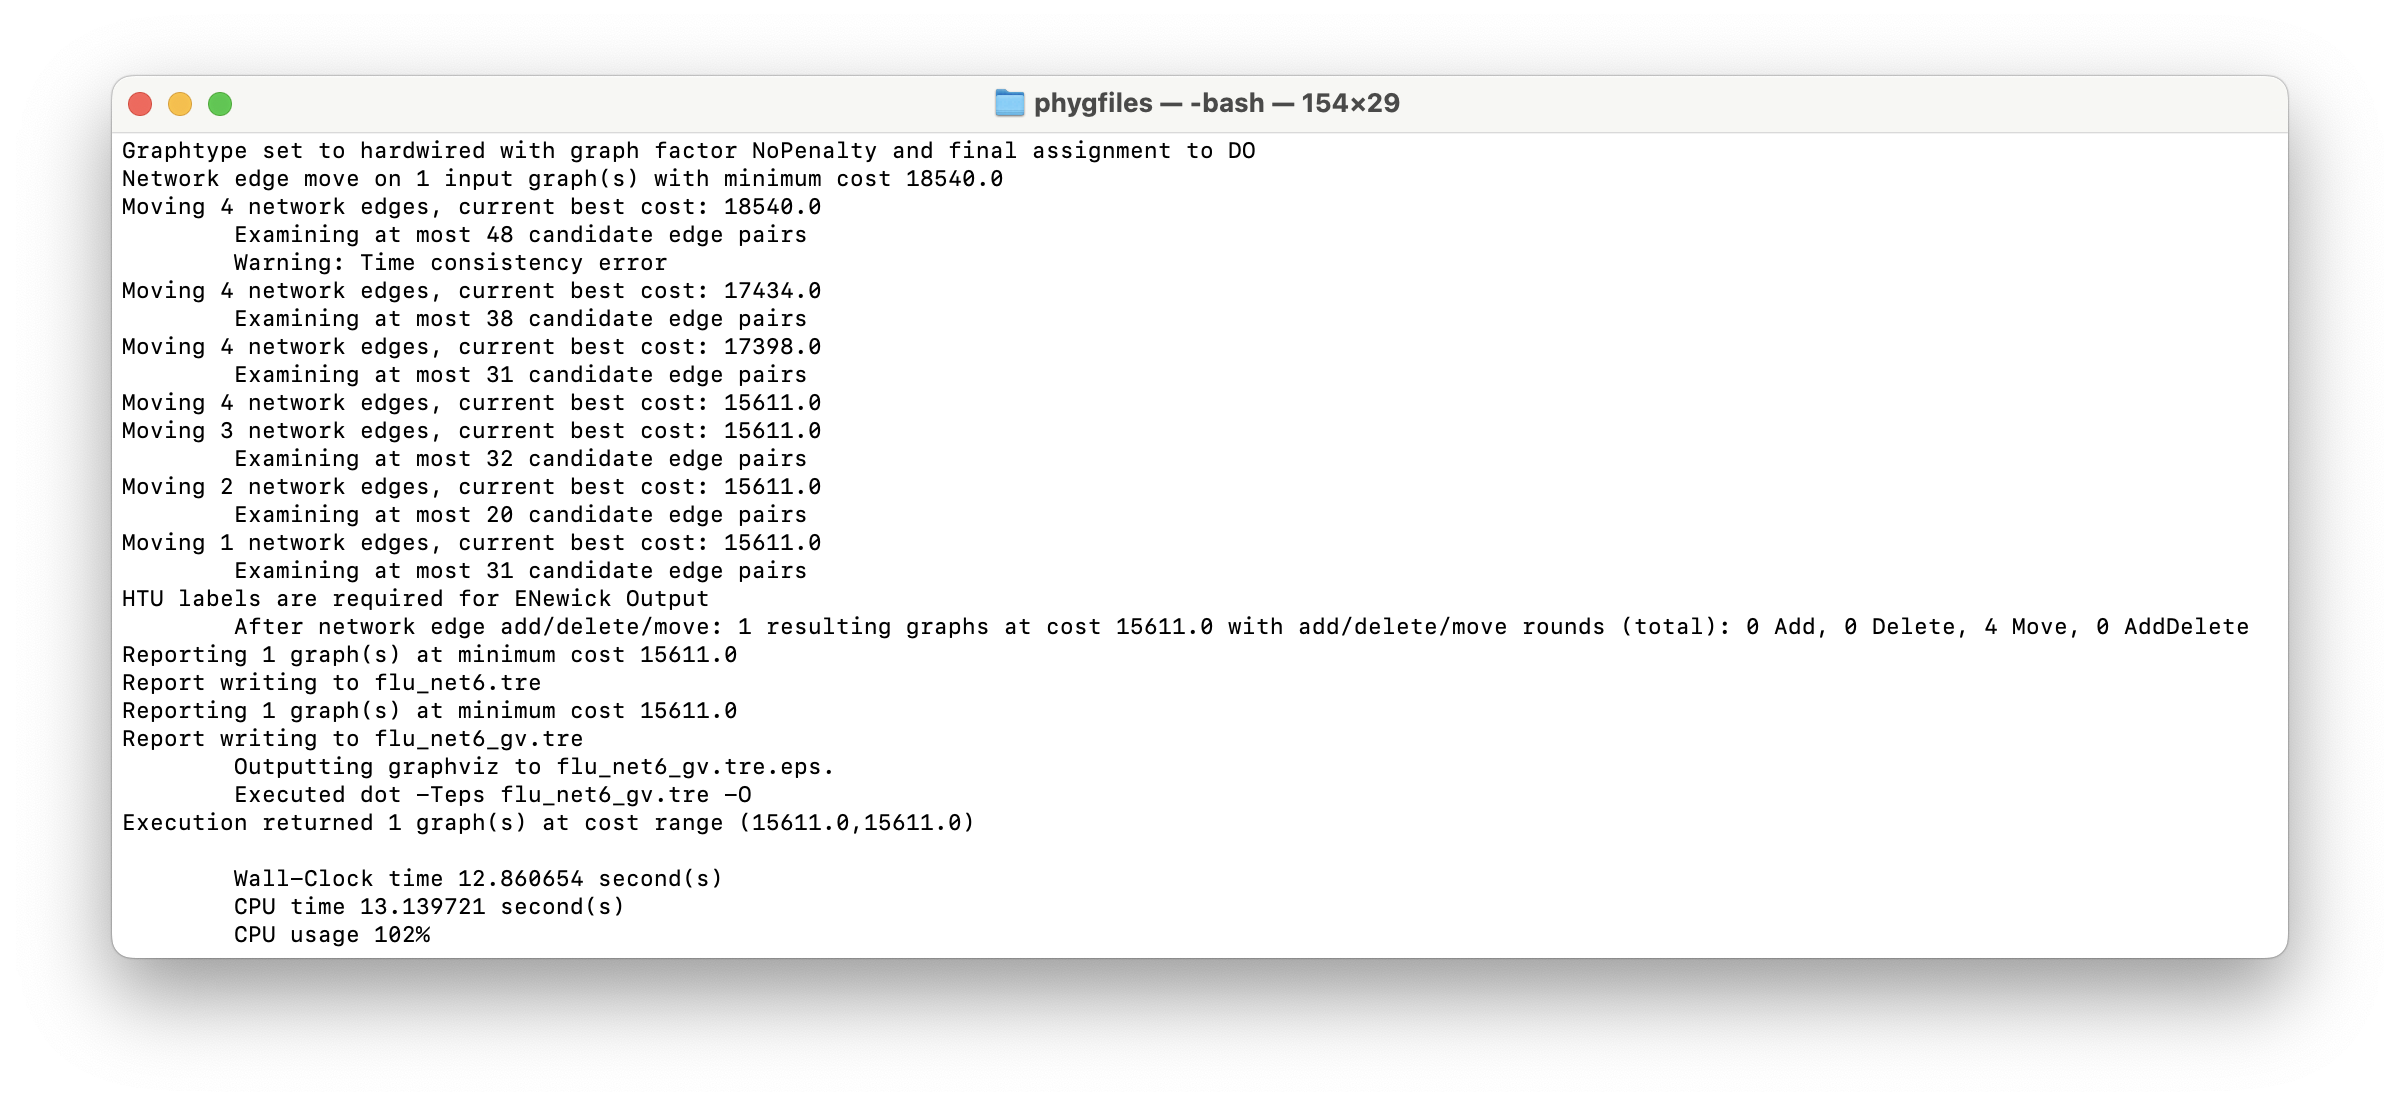
\includegraphics[width=\textwidth]{output5.png}
\caption{Output of the \textit{Terminal} window from running the script 
\textbf{``flu\_net6.pg''}.}
\label{output5}
\end{figure}

\item Scroll through the output in the \textit{Terminal} window (Figure \ref{output5}). 
Having \texttt{read} in the data files, they were then processed and the settings of 
\phyg were \texttt{set}. Notice the cost of the input graph \textbf{``flu\_net1.tre''} is 
different from when it is analyzed as a `softwired' network. The cost of the graph 
changes when it is diagnosed as a `hardwired' network. \phyg performed three 
round of moves of network edges. We can see that \phyg did four full rounds of 
moves, reduced the cost of the network from 18540 to 15611. The cost of the graph 
decreased with each move. Comparing the cost of the output graph to that found in 
(Section \ref{subsec:softnetmove}), we can see that cost of the `softwired' graph is 
14276.8125 while that of the `hardwired' graph is 15611.\\

Let's examine the reported graph files. 

\item Opening the file \textbf{``flu\_net6.tre''} in your preferred text editor. This 
ENewick file has four \textbf{\#}'s, representing the vertices (Figure \ref{tre6}). 
A single graph was reported. With \texttt{netmove} the number of network 
edges/vertices is maintained between the input and output graphs.

\begin{figure}[H]
\centering
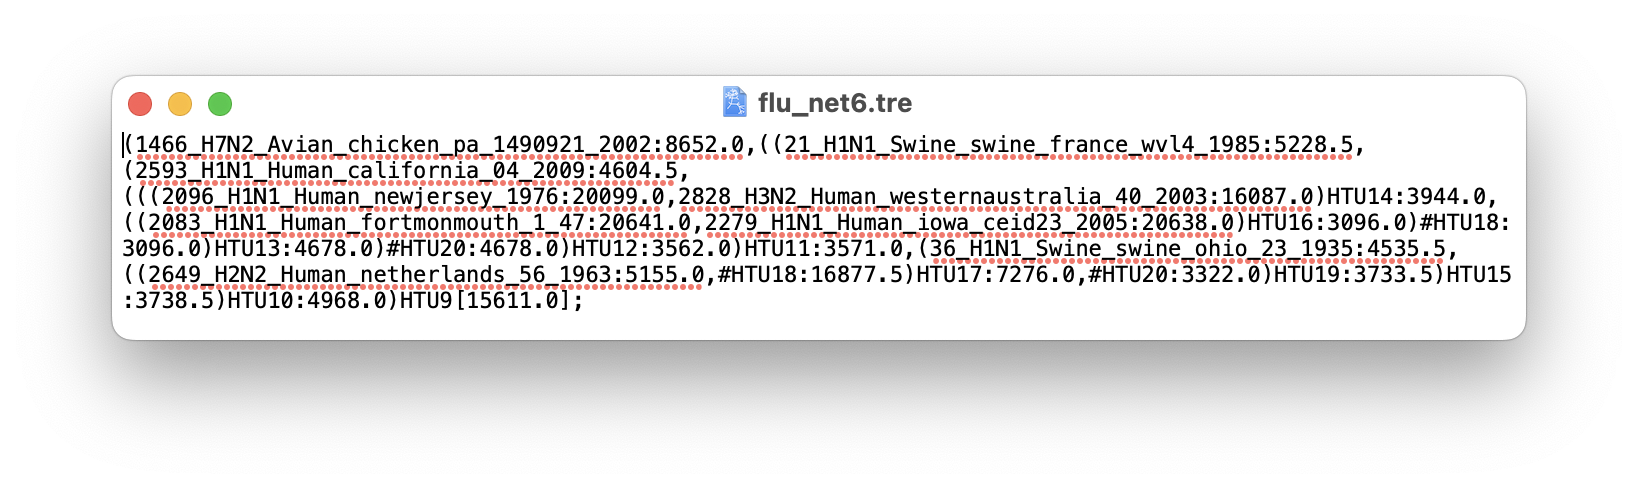
\includegraphics[width=0.8\textwidth]{tre6.png}
\caption{Output file \textbf{``flu\_net6.tre''} in ENewick graph format.}
\label{tre6}
\end{figure}

\item  Open the reported file \textbf{``flu\_net6\_gv.tre.eps''} in your preferred
visualization program (Figure \ref{eps6}). The values associated with the taxon 
names and HTUs are the branch lengths. Examining this file, we can see a four
networks leading to HTU20 and HTU18.

\begin{figure}[H]
\centering
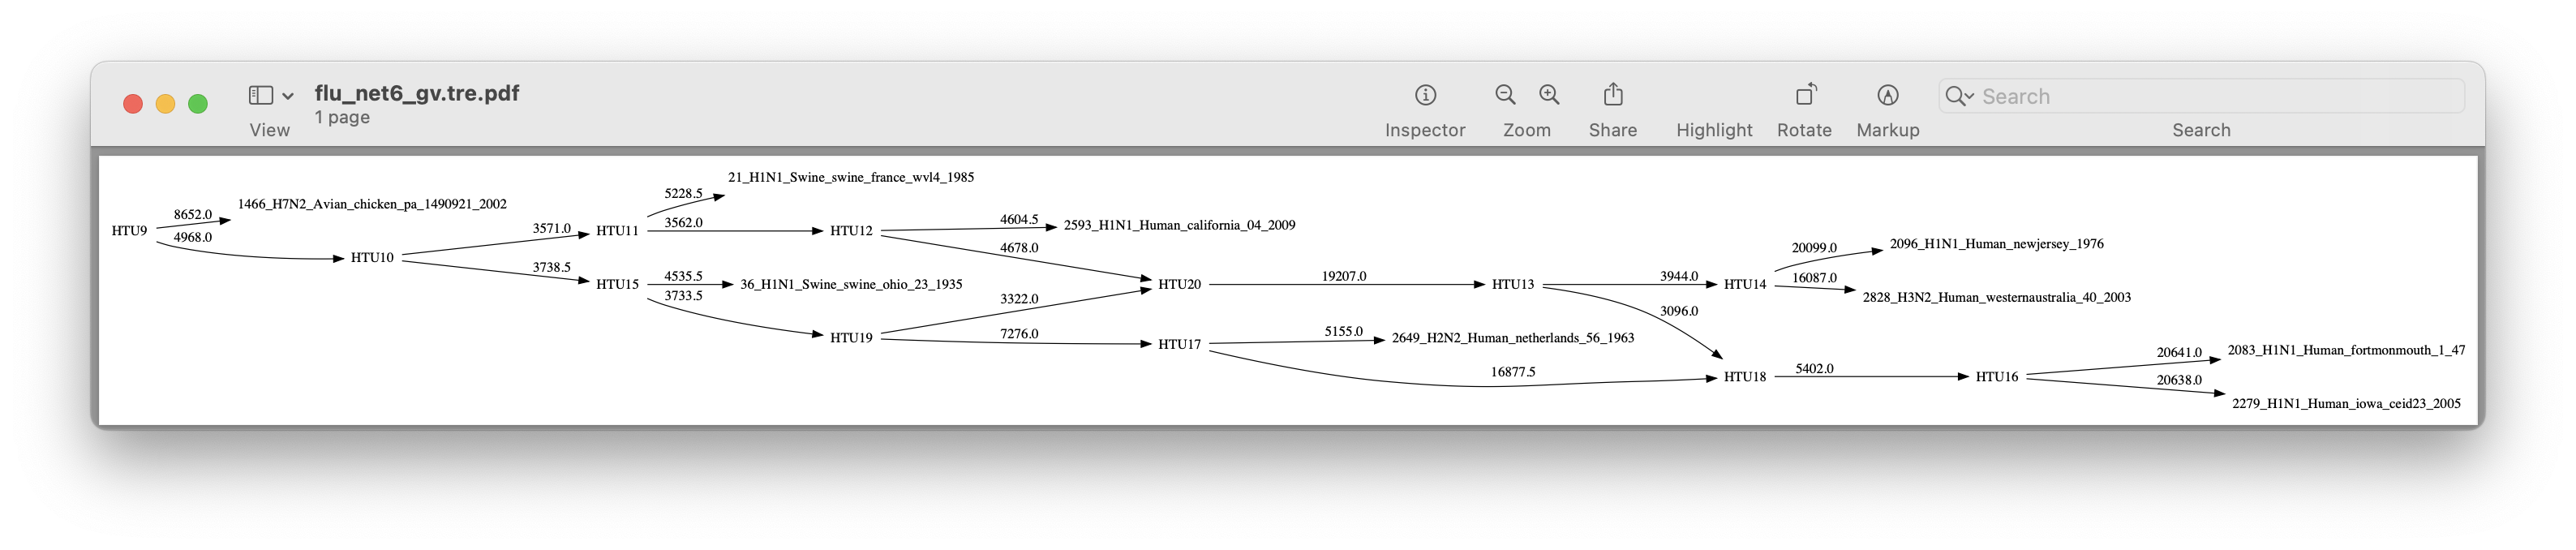
\includegraphics[width=\textwidth]{eps6.png}
\caption{Output file \textbf{"flu\_net6\_gv.tre.eps"} in eps format.}
\label{eps6}
\end{figure}

\end{enumerate}
%-------------------------------------------------------------------------------------------------------

%\printindex
\bibliography{/Users/louise/DropboxAMNH/big-refs-3.bib}
\end{document}
